In the \lephad channel, the strategy for modeling background processes where the hadronic tau is faked by a jet follows 
closely the technique described in section 5.3 of reference \cite{AlvarezPiqueras:2131232} to derive a \tauhad `fake-factor' 
in order to weight fake-\tauhad events. Fake-factors are calculated separately for SLT and LTT categories. 

The dominant source of fake-\tauhad candidates in the 2 $b$-tag signal region comes from \ttbar events, with smaller contributions from multi-jet process. 
No attempt is made to account for the negligible \Wjets process  when deriving fake-factors.
%In the 0 $b$-tag region the fake-\tauhad background is dominated by \Wjets events, while the 1 $b$-tag region has a roughly equal split of \ttbar and \Wjets events dominating the fake-\tauhad contribution. 
%Fake-factors are not derived separately for the electron and muon channels, since the probability for a jet to fake a \tauhad is 
%independent of the flavor of any accompanying charged lepton in the event. This assumption is checked and 
%no significant difference is found between the fake-factors calculated for the electron channel and those for the muon channel. 

Fake-factors ($FF$) are calculated separately for \ttbar and multi-jet, and for 1 and 3-prong \tauhad candidates. 
They are parameterised in terms of \pT(\tauhad) requiring opposite-sign lepton-tau pairs, as shown in Figures \ref{fig:SLT_FF} and \ref{fig:LTT_FF}, for the SLT and LTT categories, respectively.
For each process the $FF$ are calculated in a dedicated background enriched region. The control regions for each process are defined as follows:
 \begin{itemize}
 	\item Multi-jet: inverted lepton isolation (`tight' electrons and `medium' muons are required to fail their respective ‘loose’ isolation working points), 2 b-tag. 
 	\item \ttbar: \mbb > 150 GeV, 2 $b$-tag 
 \end{itemize}
 
A fake-\tauhad enriched sample is defined by applying the full selection defined in the signal region and in each control region, 
but requiring that the loose \tauhad is replaced by an anti-\tauhad object (failing the loose $\tau$-ID requirement, but with a RNN score > 0.01). 
In the case where the event contains more than one anti-\tauhad, one is chosen randomly. Derived variables used in the analysis,
such as the \MET, $m^{\mathrm{MMC}}_\mathrm{T}$ and \MET$\phi$ centrality are calculated in the same way as for signal events, 
but with the anti-\tauhad taking the place of the loose \tauhad candidate.

To demonstrate the purity of the desired backgrounds in the \ttbar and multi-jet control regions, 
we have included distributions of the $\tau$ $p_T$ for the control regions with the \tauhad and 
anti-\tauhad requirements, separately for 1-prong and 3-prong \tauhad.  These distributions can 
be seen in Fig.~\ref{fig:ttbarCR_1}, Fig.~\ref{fig:ttbarCR_3}, Fig.~\ref{fig:QCD_CR_1},  and Fig.~\ref{fig:QCD_CR_3}, 
where the fake contribution is taken from Monte Carlo only.  Thus, the gap between the Monte Carlo prediction and data in the multi-jet CR is attributed to multi-jet events, which are not simulated for this analysis. For simulated backgrounds, the yields can be seen in the legend.

\begin{figure}
\centering
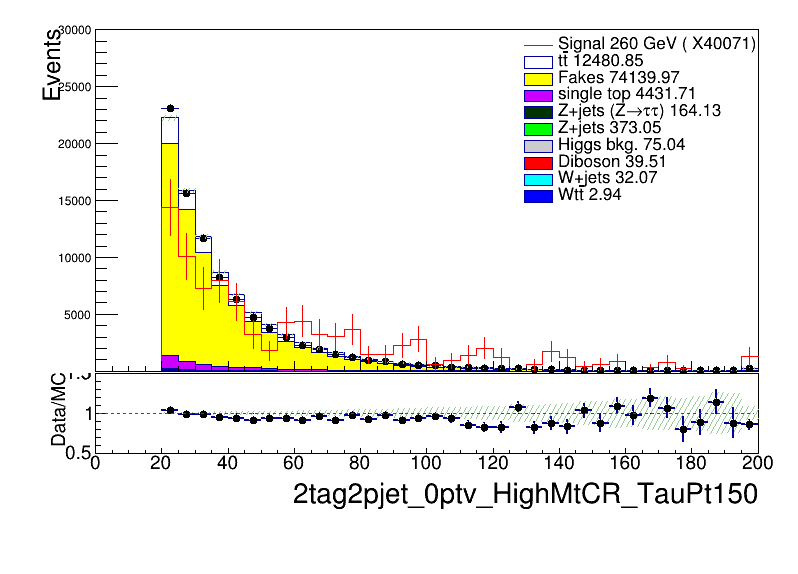
\includegraphics[width=.45\textwidth]{figures/lephadFF/SLT/2tag2pjet_0ptv_HighMtCR_TauPt150_CR_SLT_ALL_ttWeight_1.png}
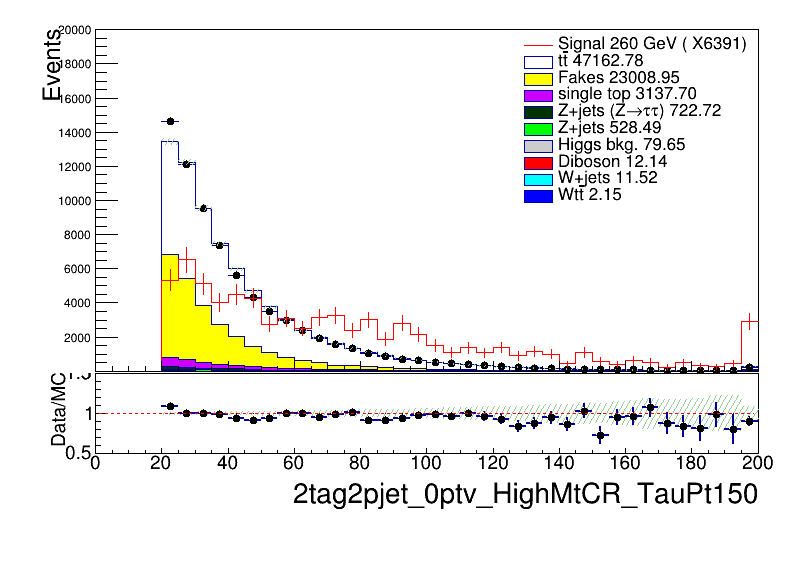
\includegraphics[width=.45\textwidth]{figures/lephadFF/SLT/2tag2pjet_0ptv_HighMtCR_TauPt150_SR_SLT_ALL_ttWeight_1.png} \\
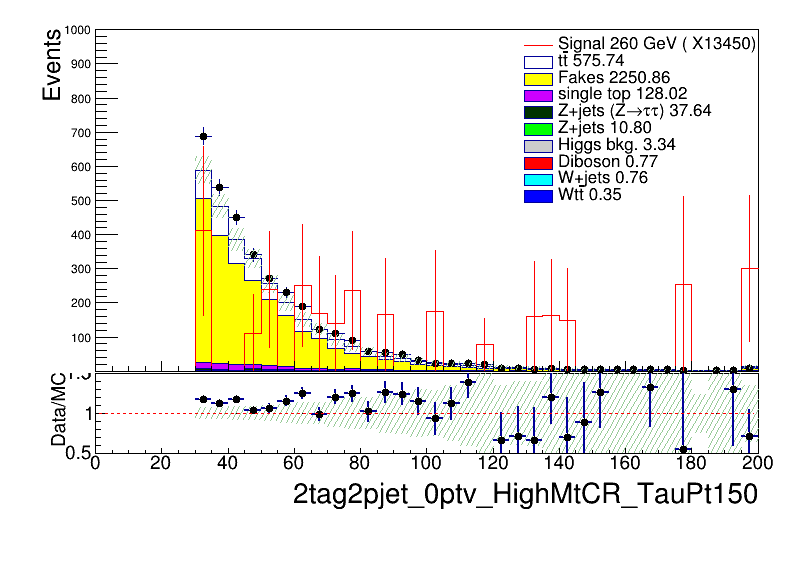
\includegraphics[width=.45\textwidth]{figures/lephadFF/LTT/2tag2pjet_0ptv_HighMtCR_TauPt150_CR_LTT_ALL_ttWeight_1.png}
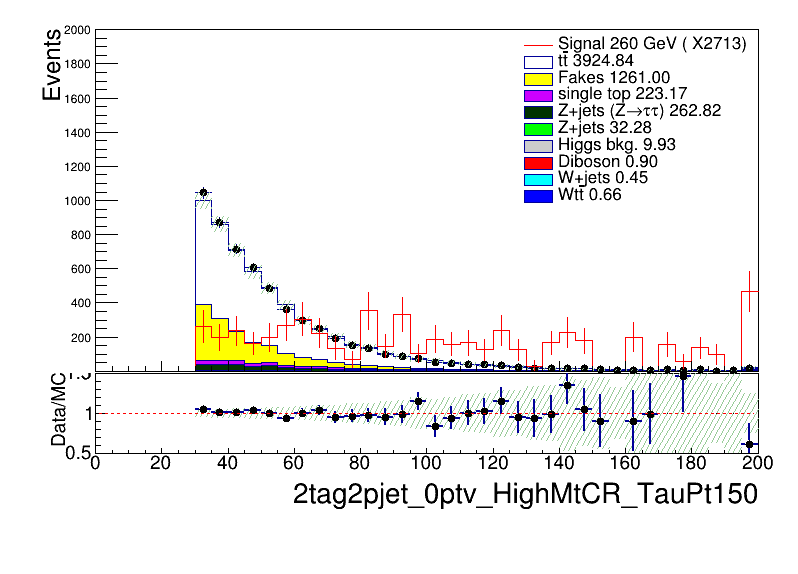
\includegraphics[width=.45\textwidth]{figures/lephadFF/LTT/2tag2pjet_0ptv_HighMtCR_TauPt150_SR_LTT_ALL_ttWeight_1.png}\\
\caption{Plots of the $\tauhad$ $p_T$ distributions for the (left) anti-\tauhad and (right) \tauhad selection for the (top) single lepton trigger and (bottom) lepton-plus-tau trigger selections in the \ttbar control region with 1-prong \tauhad.}
\label{fig:ttbarCR_1}
\end{figure} 

\begin{figure}
\centering
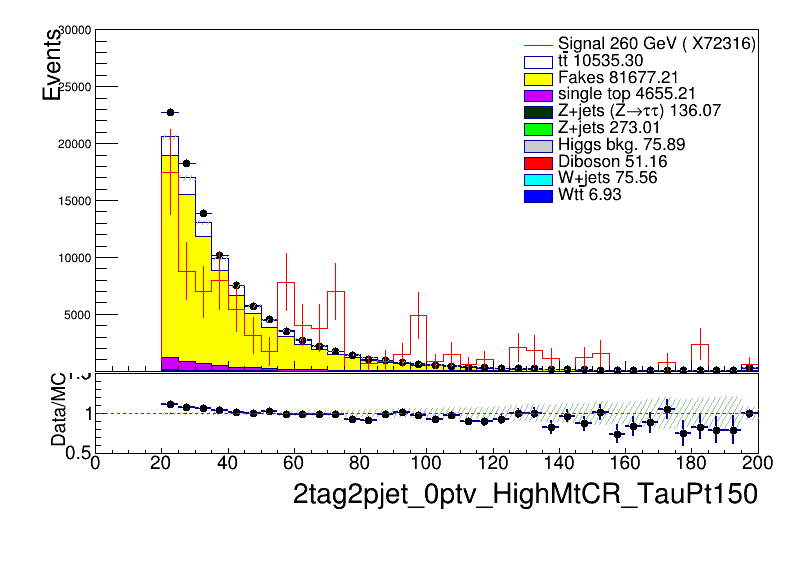
\includegraphics[width=.45\textwidth]{figures/lephadFF/SLT/2tag2pjet_0ptv_HighMtCR_TauPt150_CR_SLT_ALL_ttWeight_3.png}
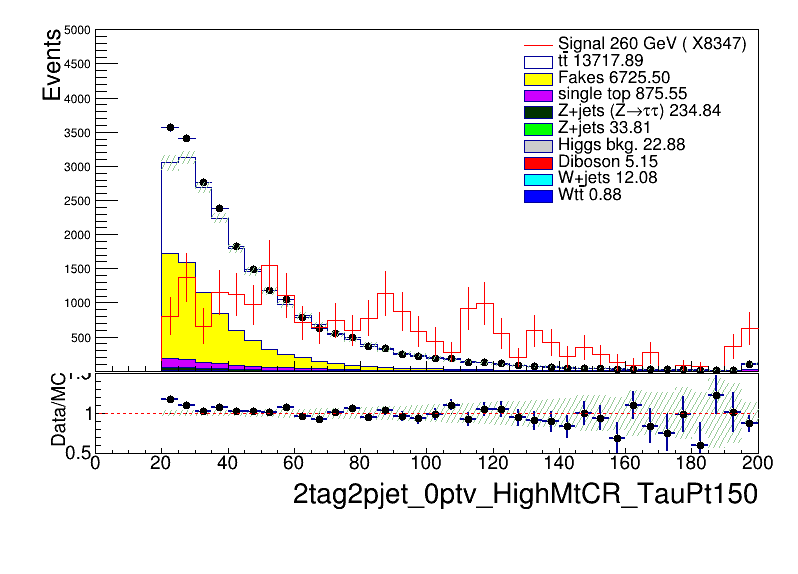
\includegraphics[width=.45\textwidth]{figures/lephadFF/SLT/2tag2pjet_0ptv_HighMtCR_TauPt150_SR_SLT_ALL_ttWeight_3.png} \\
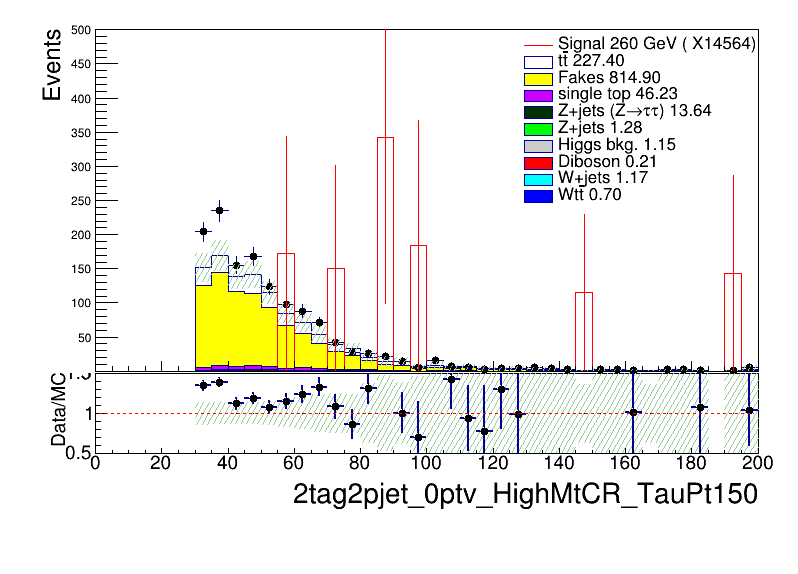
\includegraphics[width=.45\textwidth]{figures/lephadFF/LTT/2tag2pjet_0ptv_HighMtCR_TauPt150_CR_LTT_ALL_ttWeight_3.png}
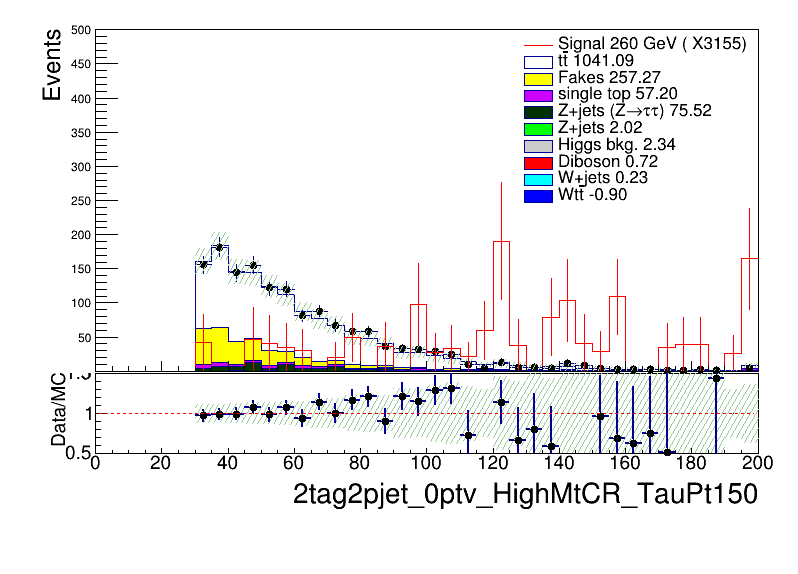
\includegraphics[width=.45\textwidth]{figures/lephadFF/LTT/2tag2pjet_0ptv_HighMtCR_TauPt150_SR_LTT_ALL_ttWeight_3.png}\\
\caption{Plots of the $\tauhad$ $p_T$ distributions for the (left) anti-\tauhad and (right) \tauhad selection for the (top) single lepton trigger and (bottom) lepton-plus-tau trigger selections in the \ttbar control region with 3-prong \tauhad.}
\label{fig:ttbarCR_3}
\end{figure}

\begin{figure}
\centering
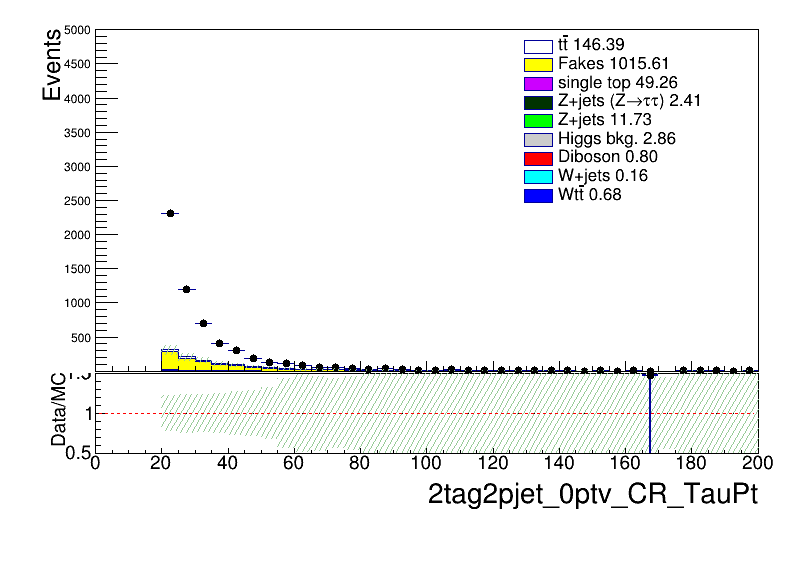
\includegraphics[width=.45\textwidth]{figures/lephadFF/SLT/2tag2pjet_0ptv_CR_TauPt_IICR_SLT_ALL_ttWeight_1.png}
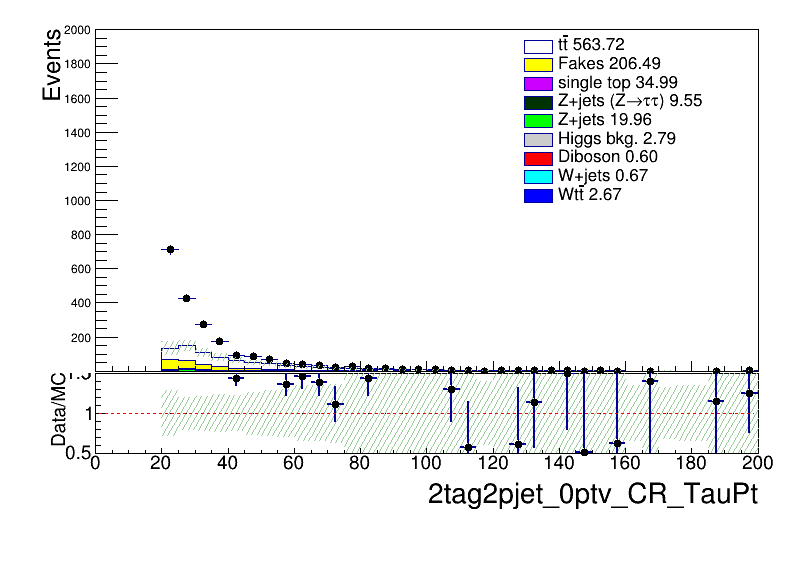
\includegraphics[width=.45\textwidth]{figures/lephadFF/SLT/2tag2pjet_0ptv_CR_TauPt_IISR_SLT_ALL_ttWeight_1.png} \\
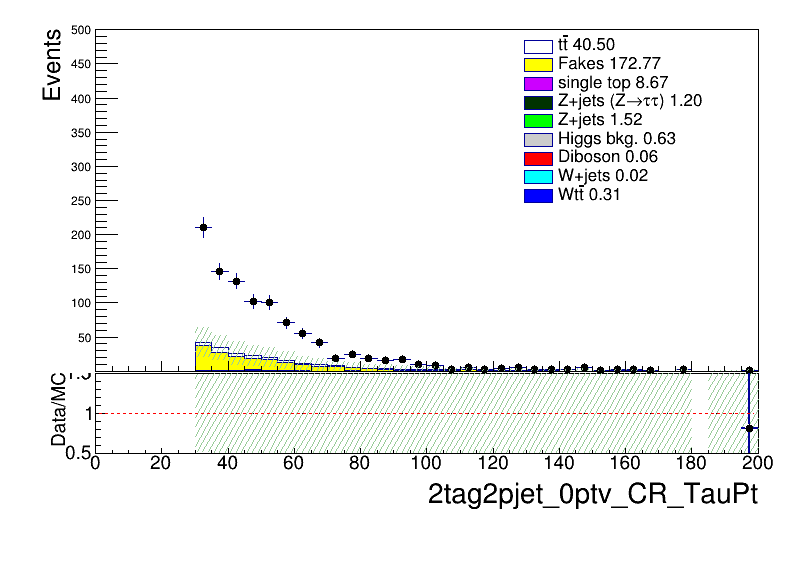
\includegraphics[width=.45\textwidth]{figures/lephadFF/LTT/2tag2pjet_0ptv_CR_TauPt_IICR_LTT_ALL_ttWeight_1.png}
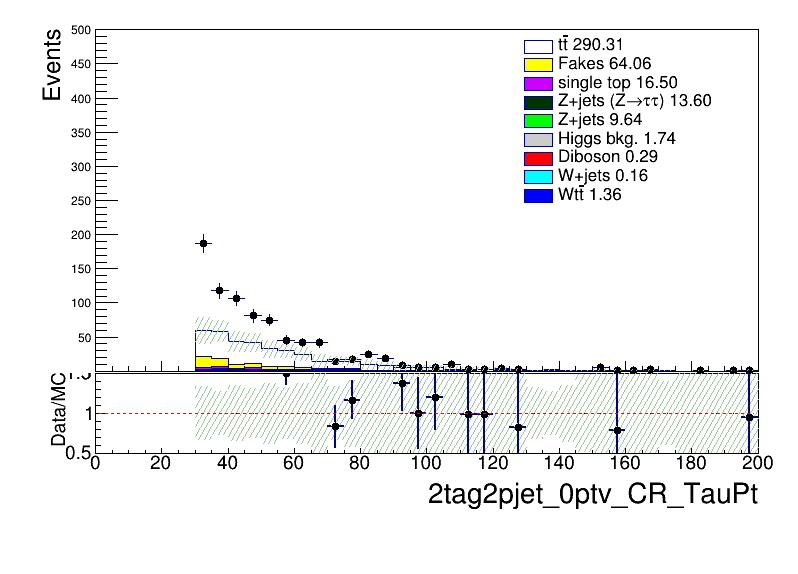
\includegraphics[width=.45\textwidth]{figures/lephadFF/LTT/2tag2pjet_0ptv_CR_TauPt_IISR_LTT_ALL_ttWeight_1.png}\\
\caption{Plots of the $\tauhad$ $p_T$ distributions for the (left) anti-\tauhad and (right) \tauhad selection for the (top) single lepton trigger and (bottom) lepton-plus-tau trigger selections in the multi-jet control region with 1-prong \tauhad.}
\label{fig:QCD_CR_1}
\end{figure}

\begin{figure}
\centering
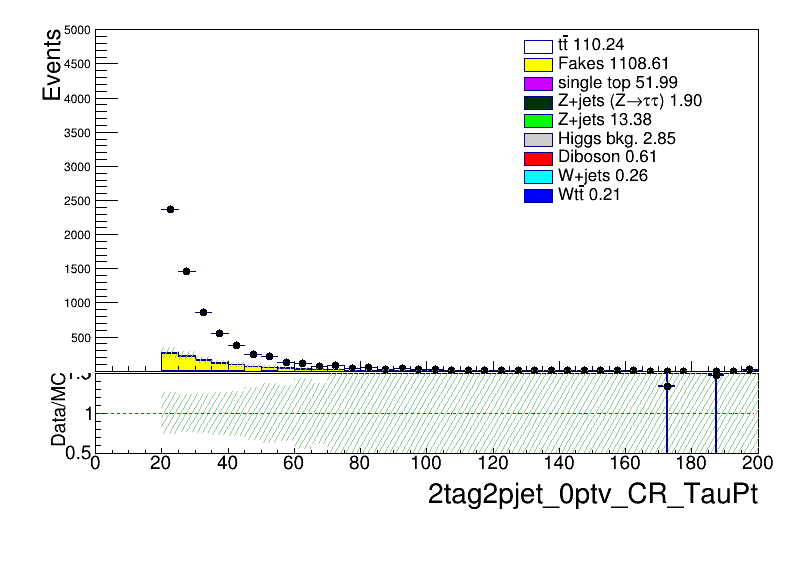
\includegraphics[width=.45\textwidth]{figures/lephadFF/SLT/2tag2pjet_0ptv_CR_TauPt_IICR_SLT_ALL_ttWeight_3.png}
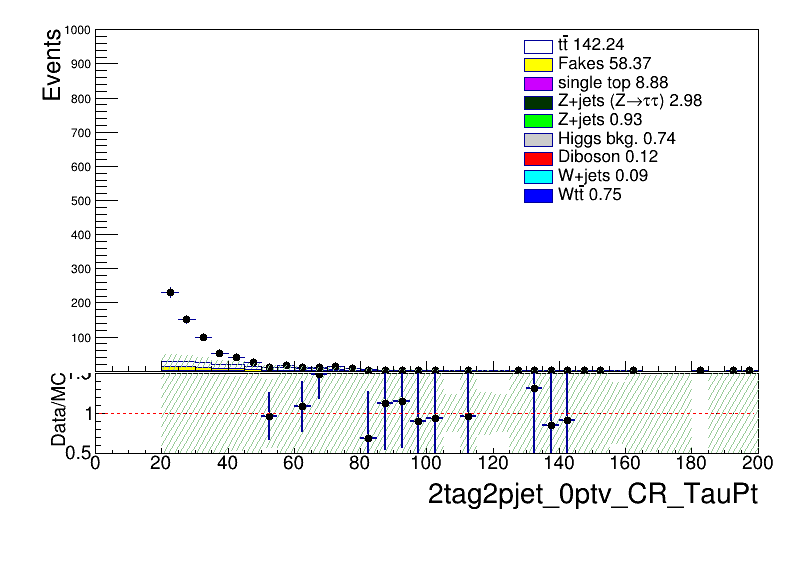
\includegraphics[width=.45\textwidth]{figures/lephadFF/SLT/2tag2pjet_0ptv_CR_TauPt_IISR_SLT_ALL_ttWeight_3.png} \\
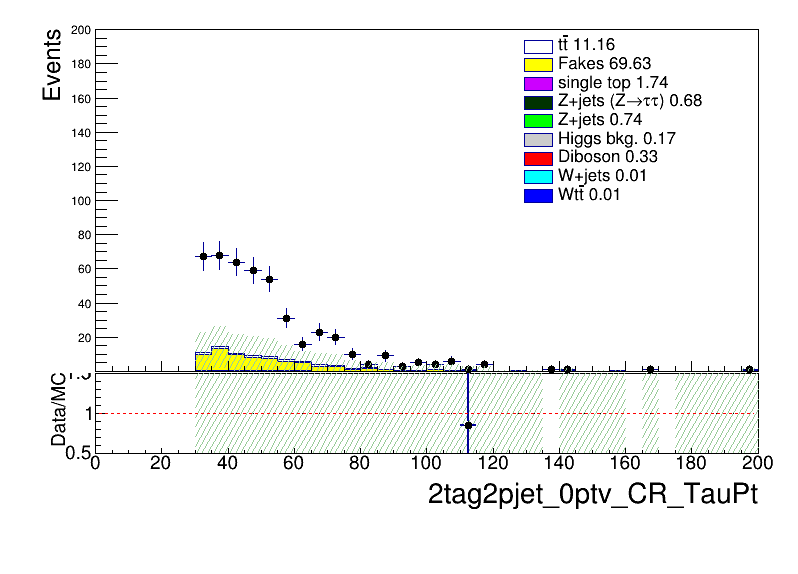
\includegraphics[width=.45\textwidth]{figures/lephadFF/LTT/2tag2pjet_0ptv_CR_TauPt_IICR_LTT_ALL_ttWeight_3.png}
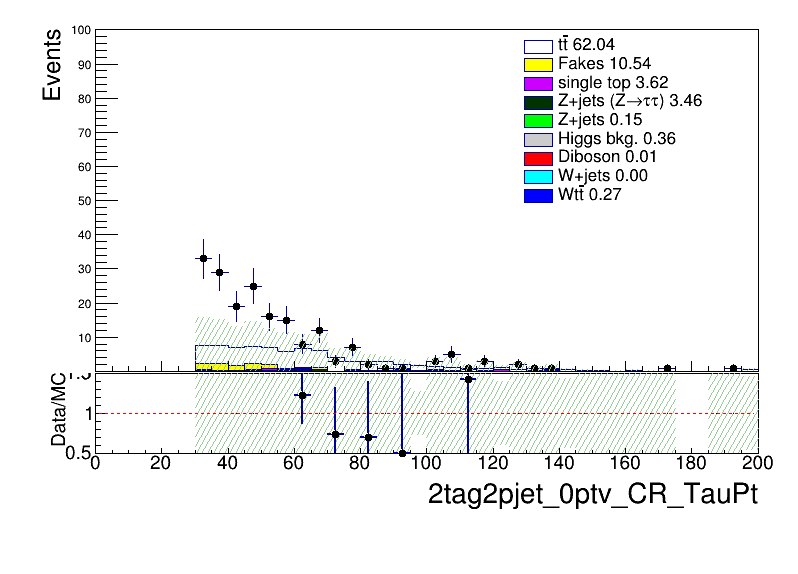
\includegraphics[width=.45\textwidth]{figures/lephadFF/LTT/2tag2pjet_0ptv_CR_TauPt_IISR_LTT_ALL_ttWeight_3.png}\\
\caption{Plots of the $\tauhad$ $p_T$ distributions for the (left) anti-\tauhad and (right) \tauhad selection for the (top) single lepton trigger and (bottom) lepton-plus-tau trigger selections in the multi-jet control region with 3-prong \tauhad.}
\label{fig:QCD_CR_3}
\end{figure}



The fake-factors are calculated as:

\begin{equation}
FF =  \frac{N(\text{loose }\tauhad)}{N(\mathrm{anti}\mhyphen\tauhad)}
\end{equation} 

where contributions from true hadronic taus and minor background processes are subtracted from 
each of the terms. Though the fake factors are parameterized only in $\tau$ $p_T$, they are also shown 
in Fig.~\ref{fig:lhFF_eta_SLT} and Fig.~\ref{fig:lhFF_eta_LTT} as a function of $\eta$, split only into barrel and endcap regions, to explore whether there is 
a significant dependence on $\tau$ $\eta$. There is no clear trend, which is why the fake factors are not parameterized in 
terms of $\eta$.

\begin{figure}
\centering
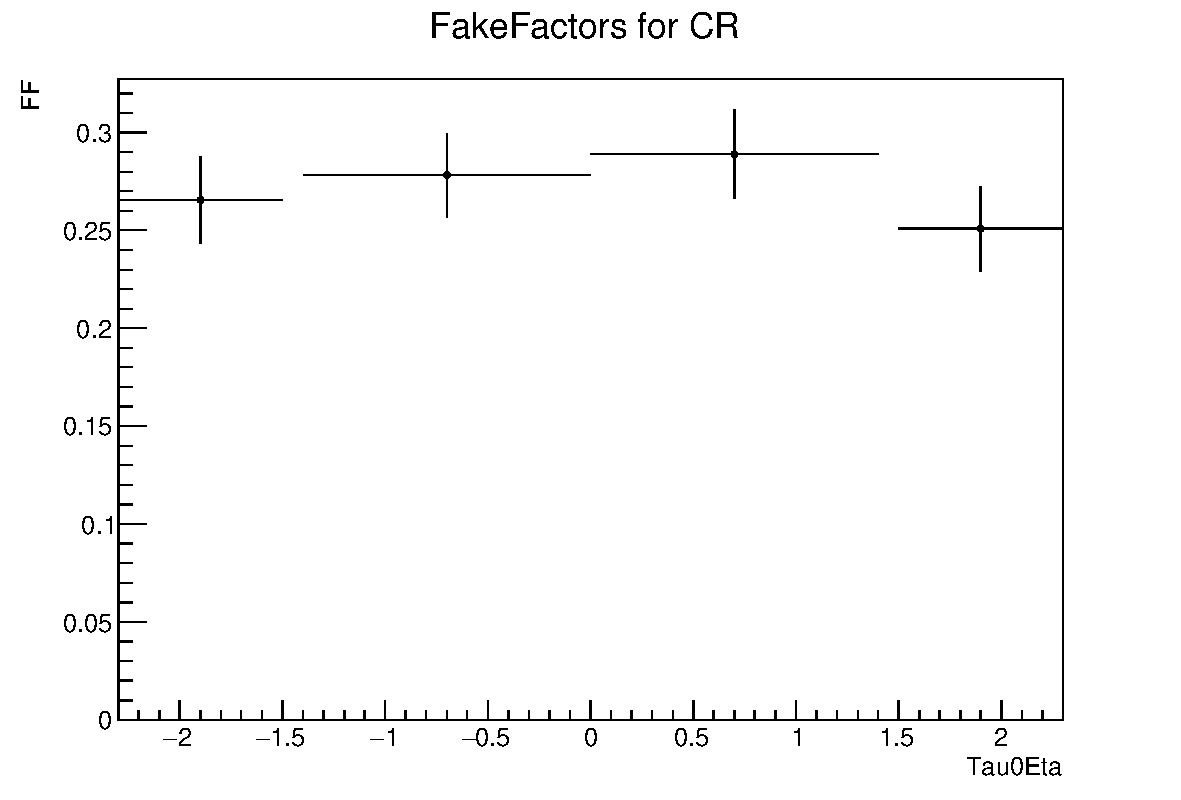
\includegraphics[width=.4\textwidth]{figures/lephadFF/SLT/FF_All_Preselection_Np1_CR_2tag_Tau0Eta}
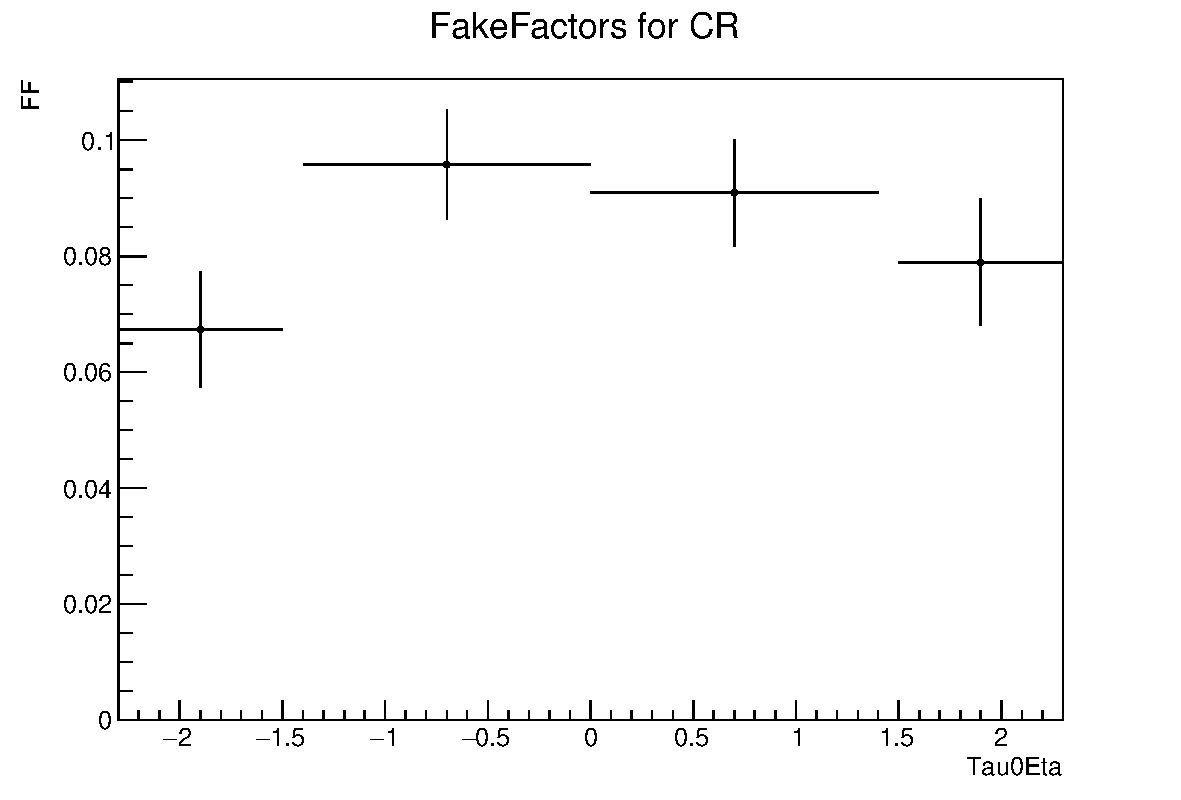
\includegraphics[width=.4\textwidth]{figures/lephadFF/SLT/FF_All_Preselection_Np3_CR_2tag_Tau0Eta} \\
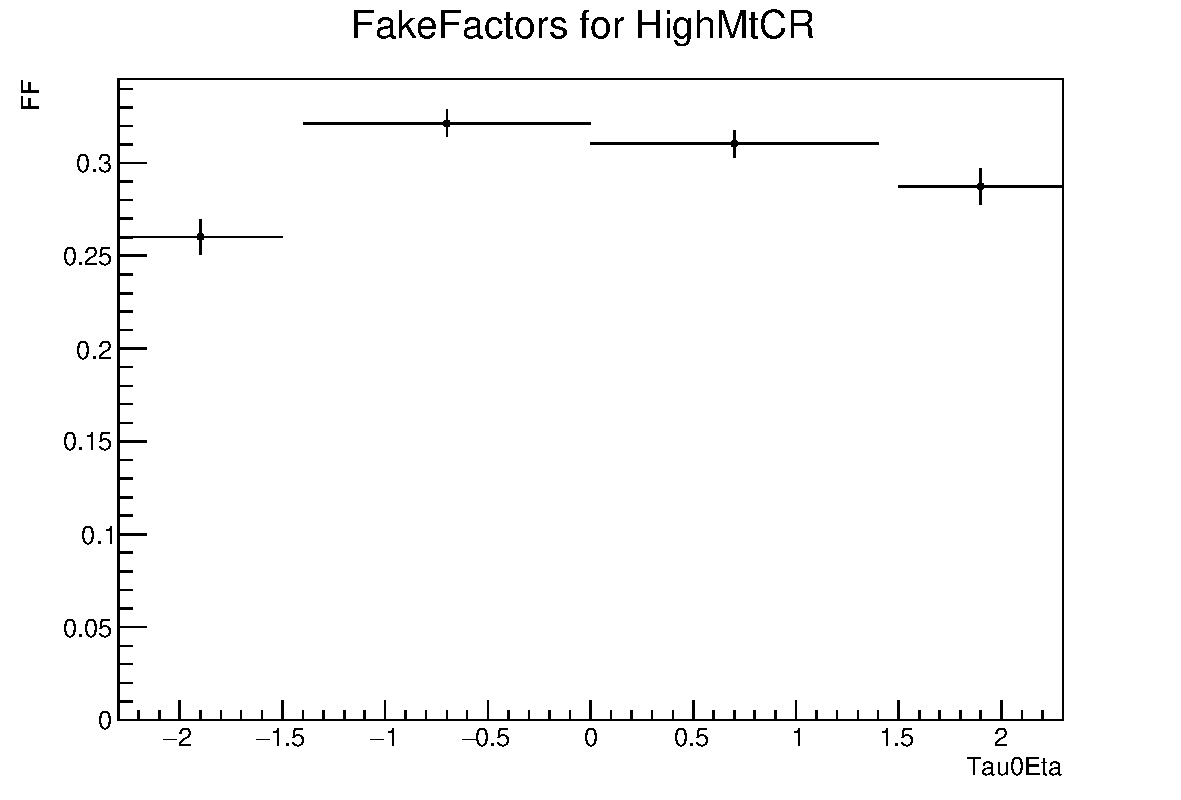
\includegraphics[width=.4\textwidth]{figures/lephadFF/SLT/FF_All_Preselection_Np1_HighMtCR_2tag_Tau0Eta}
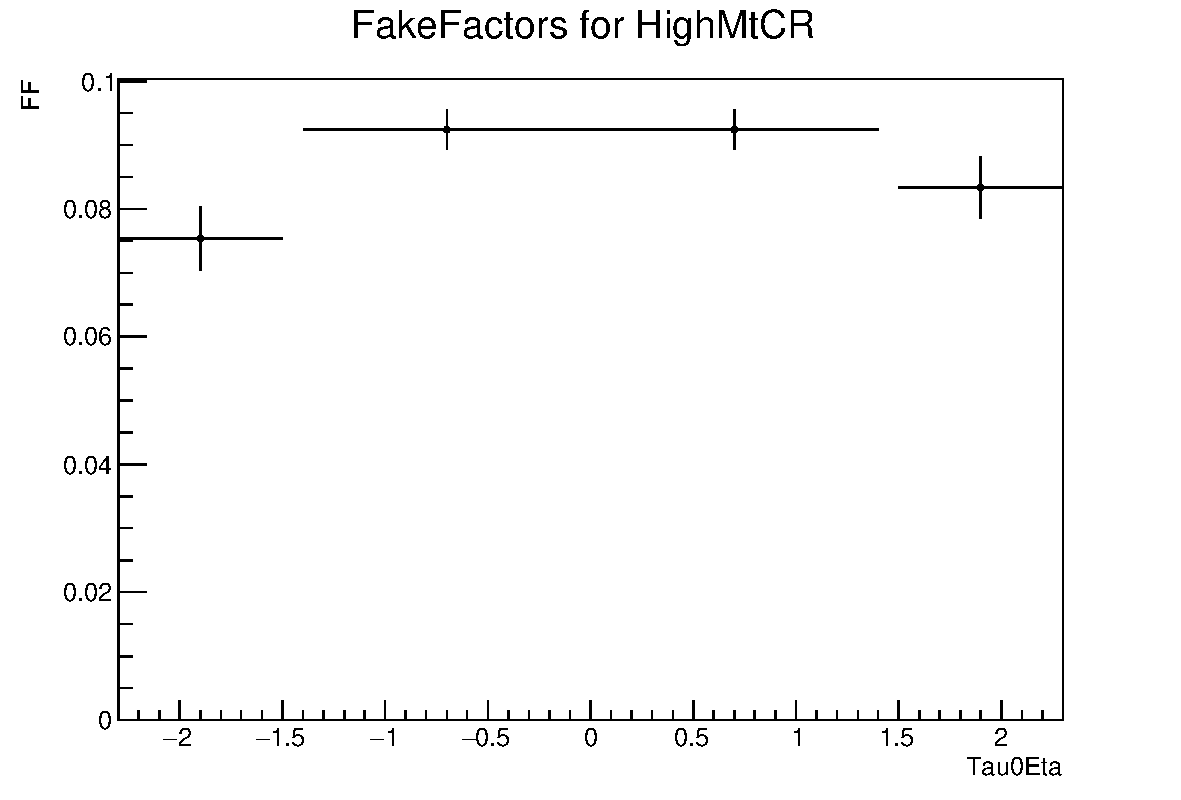
\includegraphics[width=.4\textwidth]{figures/lephadFF/SLT/FF_All_Preselection_Np3_HighMtCR_2tag_Tau0Eta}\\
\caption{Fake-factors as a function of $\eta$ for 1-prong (left) and 3-prong (right) \tauhad candidates for multi-jet (top) and \ttbar processes (bottom) for the \lephad SLT category. No significant trend is observed.}
\label{fig:lhFF_eta_SLT}
\end{figure}

\begin{figure}
\centering
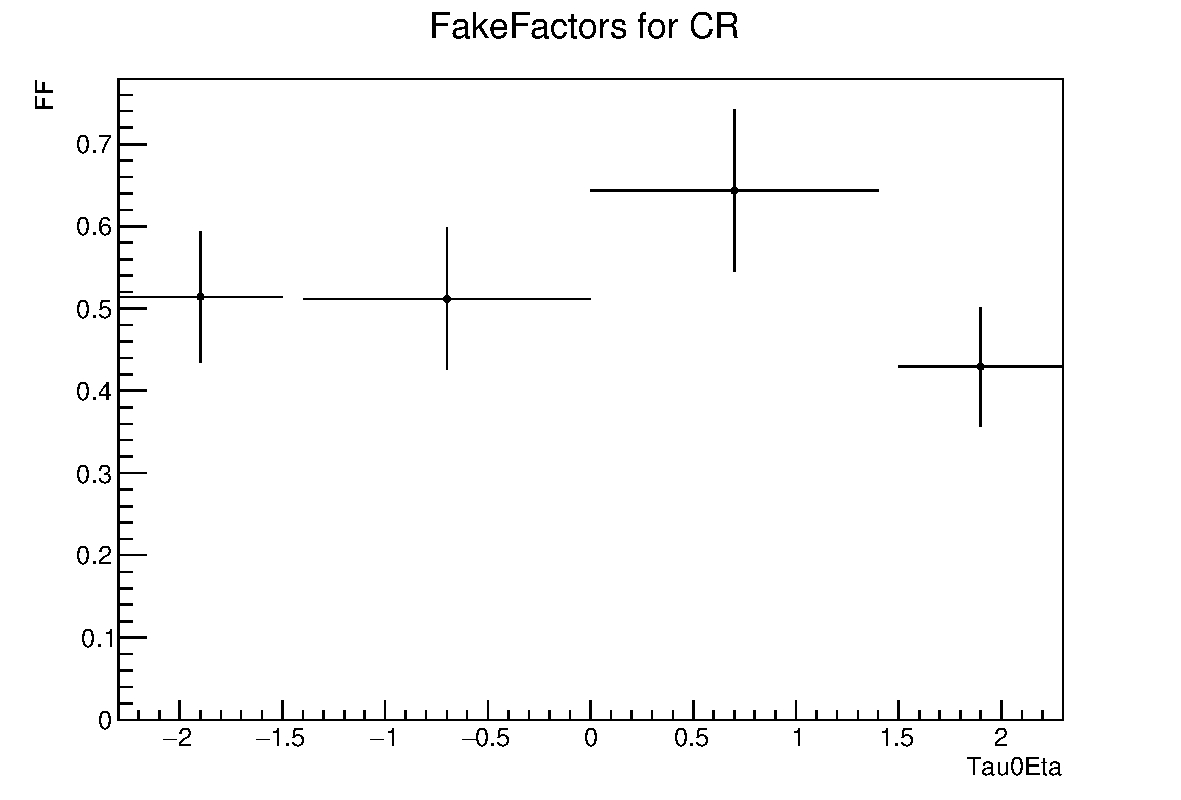
\includegraphics[width=.4\textwidth]{figures/lephadFF/LTT/FF_All_Preselection_Np1_CR_2tag_Tau0Eta}
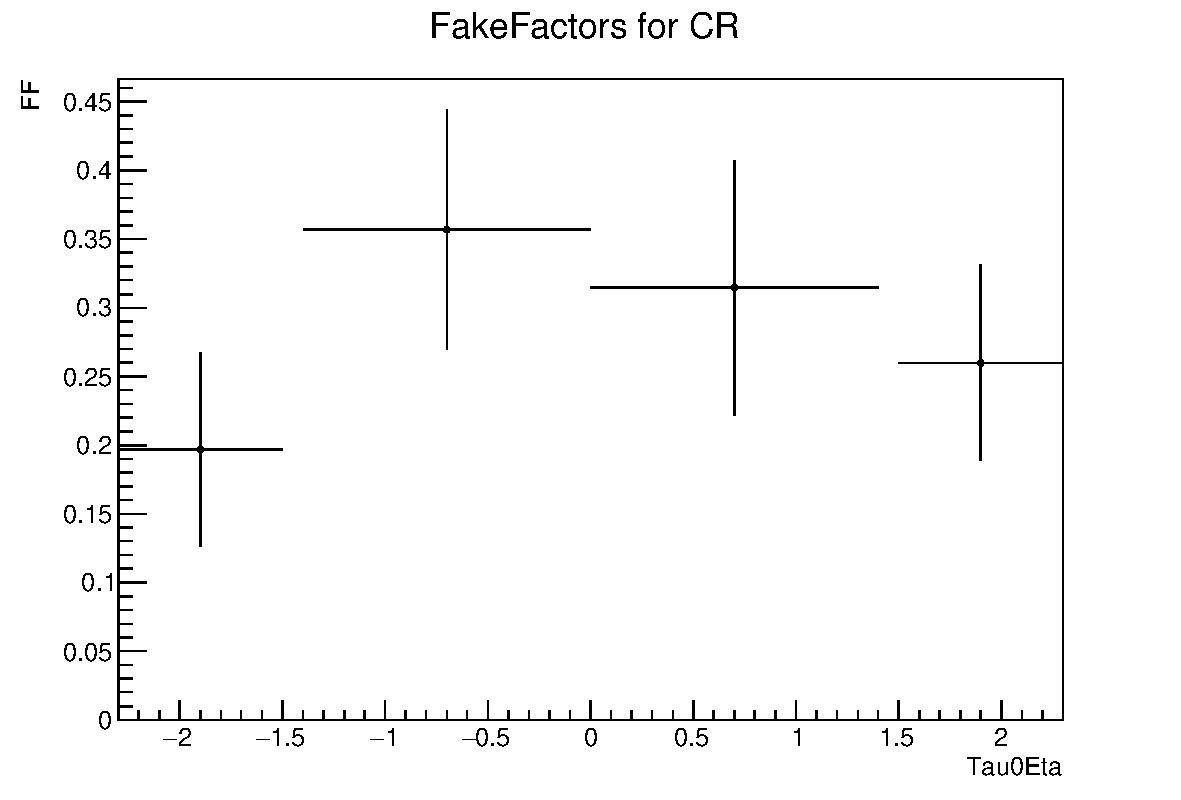
\includegraphics[width=.4\textwidth]{figures/lephadFF/LTT/FF_All_Preselection_Np3_CR_2tag_Tau0Eta} \\
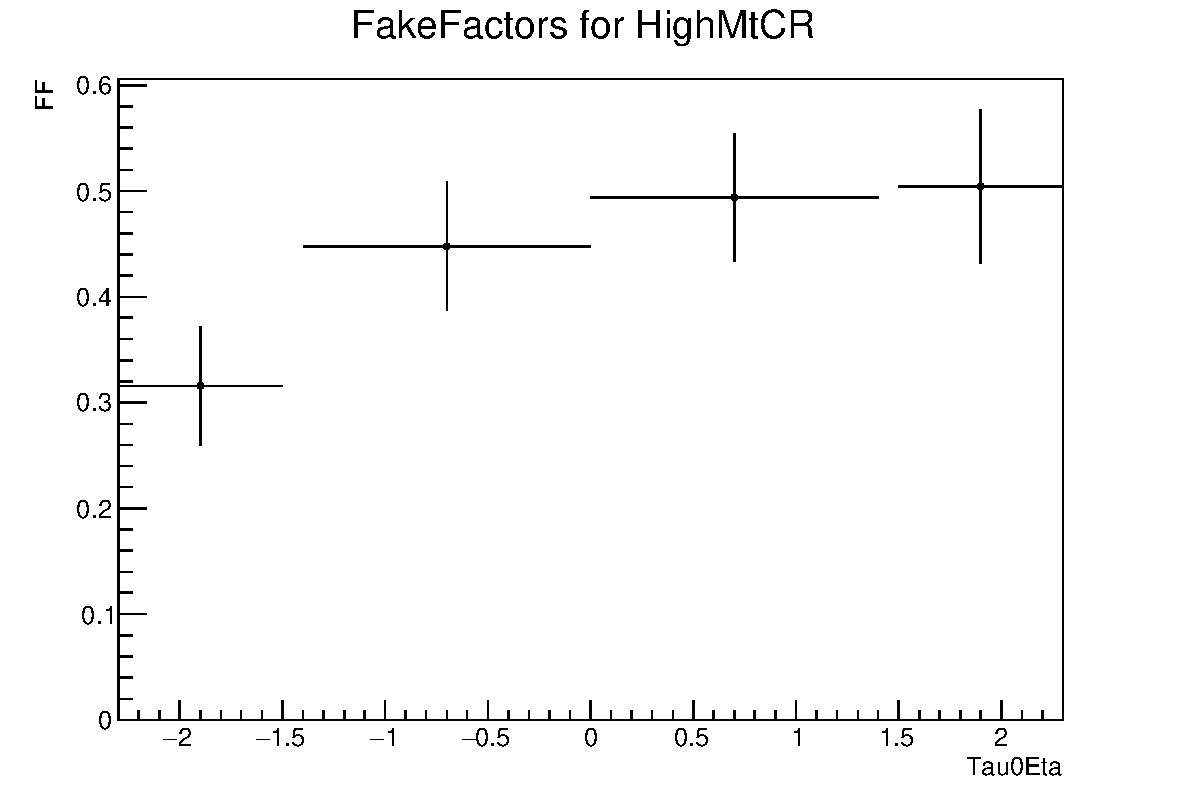
\includegraphics[width=.4\textwidth]{figures/lephadFF/LTT/FF_All_Preselection_Np1_HighMtCR_2tag_Tau0Eta}
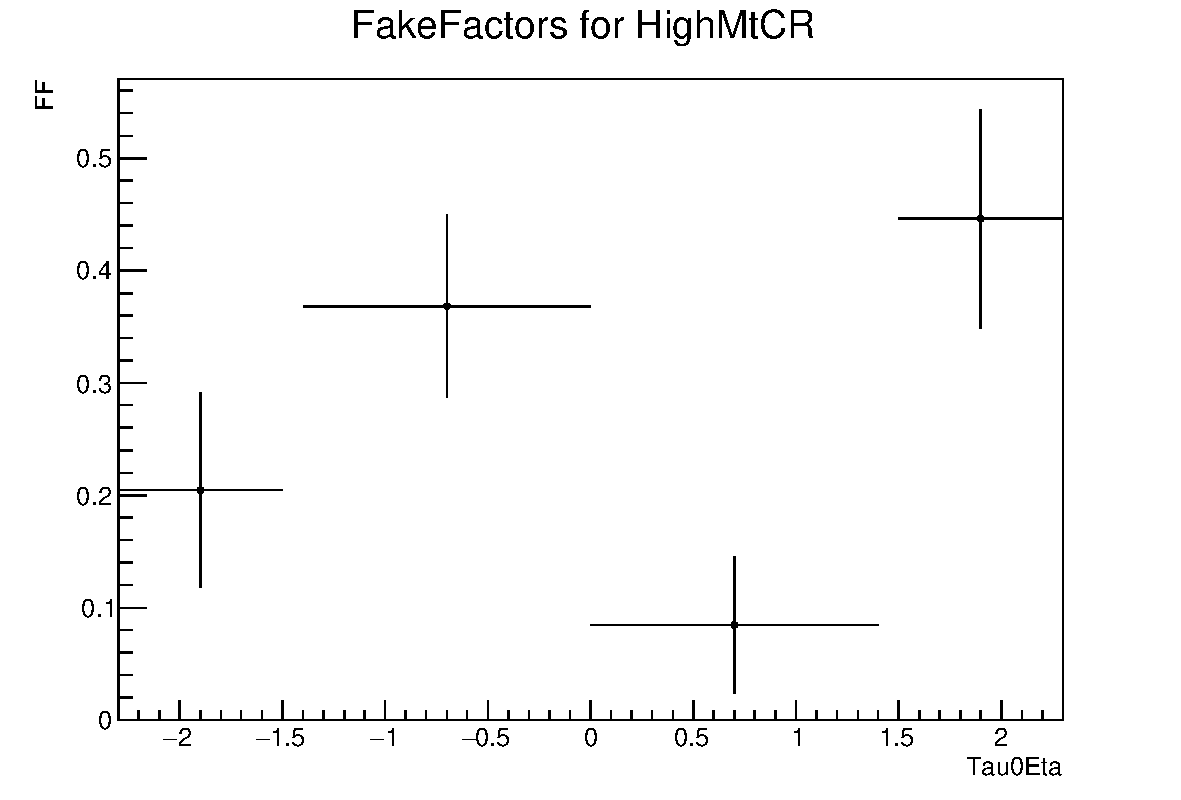
\includegraphics[width=.4\textwidth]{figures/lephadFF/LTT/FF_All_Preselection_Np3_HighMtCR_2tag_Tau0Eta}\\
\caption{Fake-factors as a function of $\eta$ for 1-prong (left) and 3-prong (right) \tauhad candidates for multi-jet (top) and \ttbar processes (bottom) for the \lephad LTT category. No significant trend is observed.}
\label{fig:lhFF_eta_LTT}
\end{figure}


Individual fake-factors for each process (multi-jet, \ttbar) are then used to provide a combined fake-factor. 
The combined $FF$ is then applied to anti-tau samples where the full signal selection is otherwise applied, 
in order to correct the normalisation and estimate the fake-\tauhad background in the regular (ID-tau) signal region. 
The combined fake-factor is defined as:

\begin{equation}
FF(\mathrm{comb}) = FF(\mathrm{QCD}) \times \mathrm{r}_{\mathrm{QCD}} + FF(\ttbar) \times (1 - \mathrm{r}_{\mathrm{QCD}}) 
\end{equation} 

where $\mathrm{r}_{\mathrm{QCD}}$ is measured as a function of the \tauhad \pT and defined as the fraction of multi-jet events in the anti-tau signal region:

\begin{equation}
\mathrm{r}_{\mathrm{QCD}} = \frac{N(\mathrm{multi\mhyphen jet, data})} {N(\mathrm{data}) - N(\mathrm{true}~\tauhad, \mathrm{MC})}
\end{equation} 

where all predicted MC events in the anti-\tauhad region are subtracted from the number of data events, $N(\mathrm{data})$, regardless of whether or not they contain a true \tauhad:

\begin{equation}
N(\mathrm{multi\mhyphen jet, data}) = N(\mathrm{data}) - N(\mathrm{true}~\tauhad, \mathrm{MC} + \mathrm{fake}~\tauhad, \mathrm{MC})
\end{equation} 

The $N(\mathrm{multi\mhyphen jet, data})$ is calculated by subtracting all background contributions apart from multi-jet, regardless of whether they contain fake or true-\tauhad candidates, from the data in the anti-ID tau region. 
The subtracted backgrounds are taken from the MC predictions. In graphical form, the various control regions where the fake factors are measured and applied can be seen in Fig.~\ref{fig:CombFFMethod}.
 
\begin{figure}
\centering
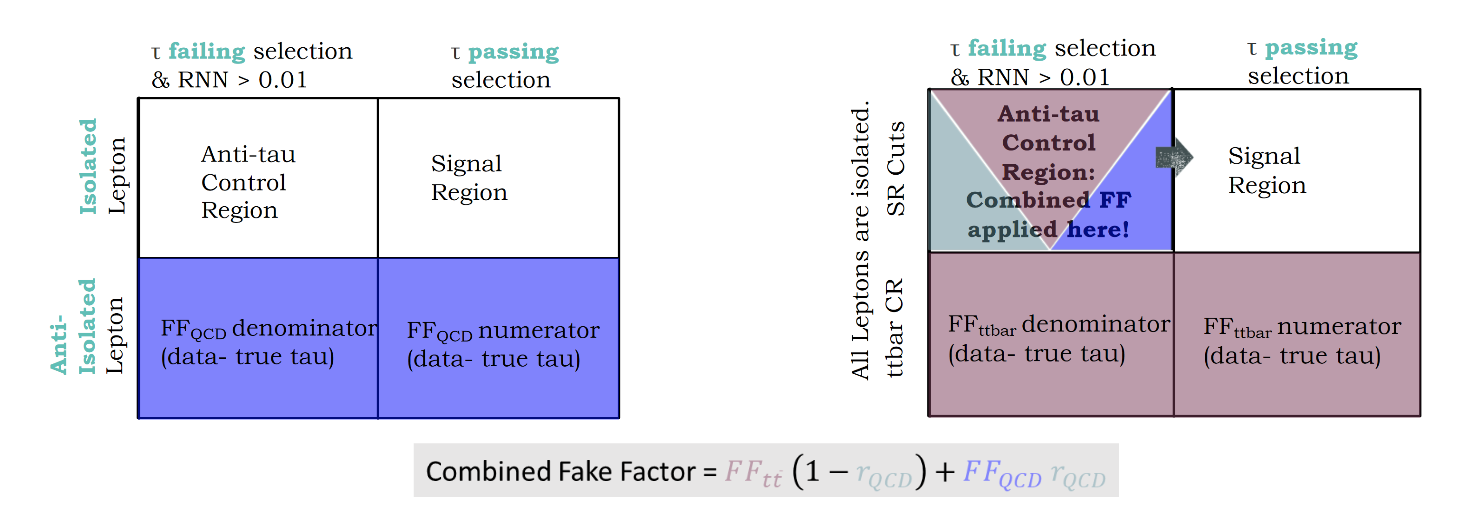
\includegraphics[width=.9\textwidth]{figures/lephadFF/CombinedFFMethod.png}
\caption{Graphical representation of the Combined Fake Factor Method}
\label{fig:CombFFMethod}
\end{figure}


It was observed that known mismodeling in the \ttbar\ background can cause issues in the calculation of the fake factors, most notably making them eventually become negative at very high values of $\tau$ transverse momentum.  For this reason, the \ttbar\ background is reweighted when it is subtracted in the calculation and application of fake factors.  This reweighting method is described in Appendix~\ref{subsec:appendix_bkg_ttbar_reweighting}.  The difference between the background estimation achieved with and without this \ttbar\ reweighting will be taken as an additional uncertainty on the method. The FF comparison with \ttbar-reweighting vs. no-\ttbar-reweighting is shown in Fig. \ref{fig:FFRW} for a demonstration of this uncertainty. This reweighting is applied in all the control regions used for the calculation of the combined fake factors, though it has the largest impact on the \ttbar fake factor contribution. 

The $\mathrm{r}_{\mathrm{QCD}}$ factor is computed both for $e\tauhad$ and $\mu\tauhad$ channels, since the QCD contents are different for them.
The parameterized $\mathrm{r}_{\mathrm{QCD}}$ as a function of \pT(\tauhad) for 1-prong and 3-prong \tauhad candidates in $e\tauhad$ and $\mu\tauhad$ channels 
are shown in Fig \ref{fig:SLT_rQCD} for the SLT category and in Fig. \ref{fig:LTT_rQCD} for the LTT category. The nature of the combined fake factor requires the same binning in both fake factors and the multi-jet fraction, but it is clear by looking at the multi-jet fraction that the \ttbar fake factor is dominant across the full $p_T$ range.  Thus, the binning of the fake factor was selected based on the \ttbar fake factor.  The binning was chosen by first looking at the fake factors as a function of $p_T$ in 5 GeV bins, and then merging statistically consistent bins until the trend was fully described. This binning is not optimal for the multi-jet fake factor and results in some binning artifact shapes at mid and high $p_T$.  As the multi-jet fake factor contributes negligibly to the combined fake factor at higher $p_T$, these binning artifacts are not seen as a significant problem.  It has been confirmed that it is possible to instead choose the binning based only on the statistics of the multi-jet fake factors, which results in a smooth trend in these fake factors.

\begin{figure}
\centering
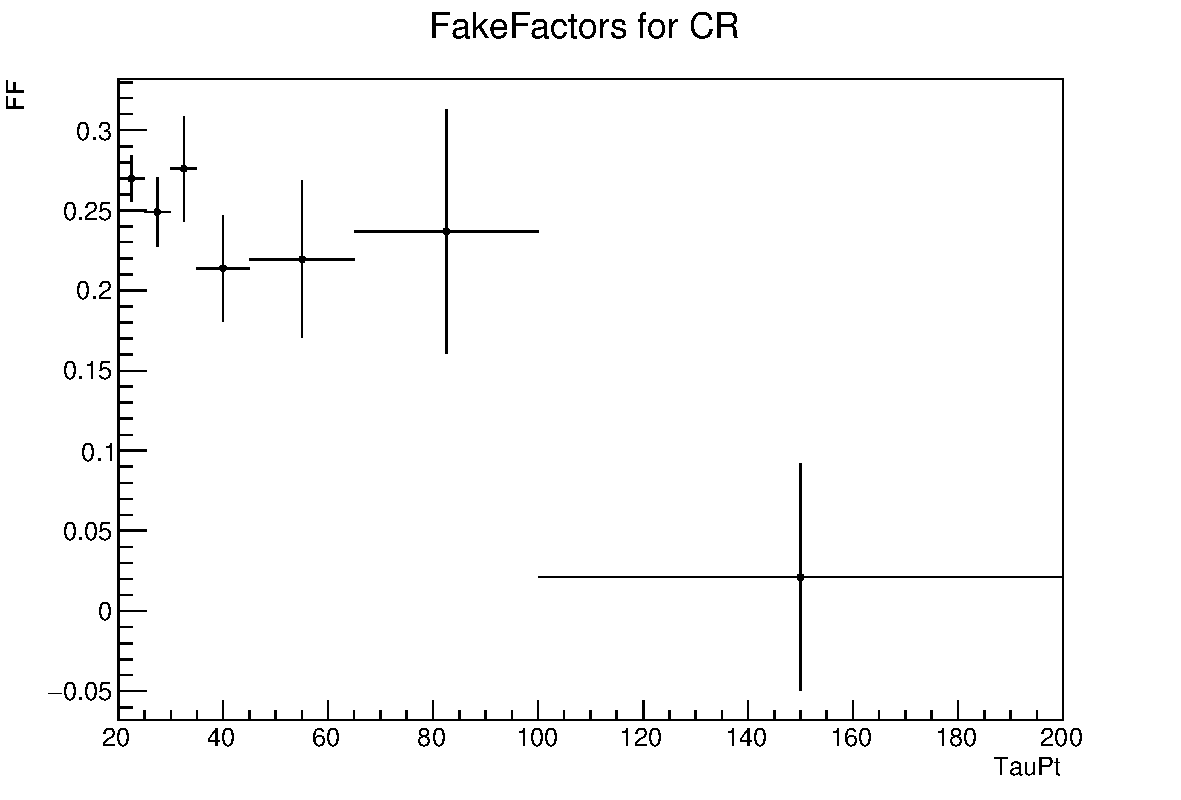
\includegraphics[width=.4\textwidth]{figures/lephadFF/SLT/FF_All_Preselection_Np1_CR_2tag_TauPt}
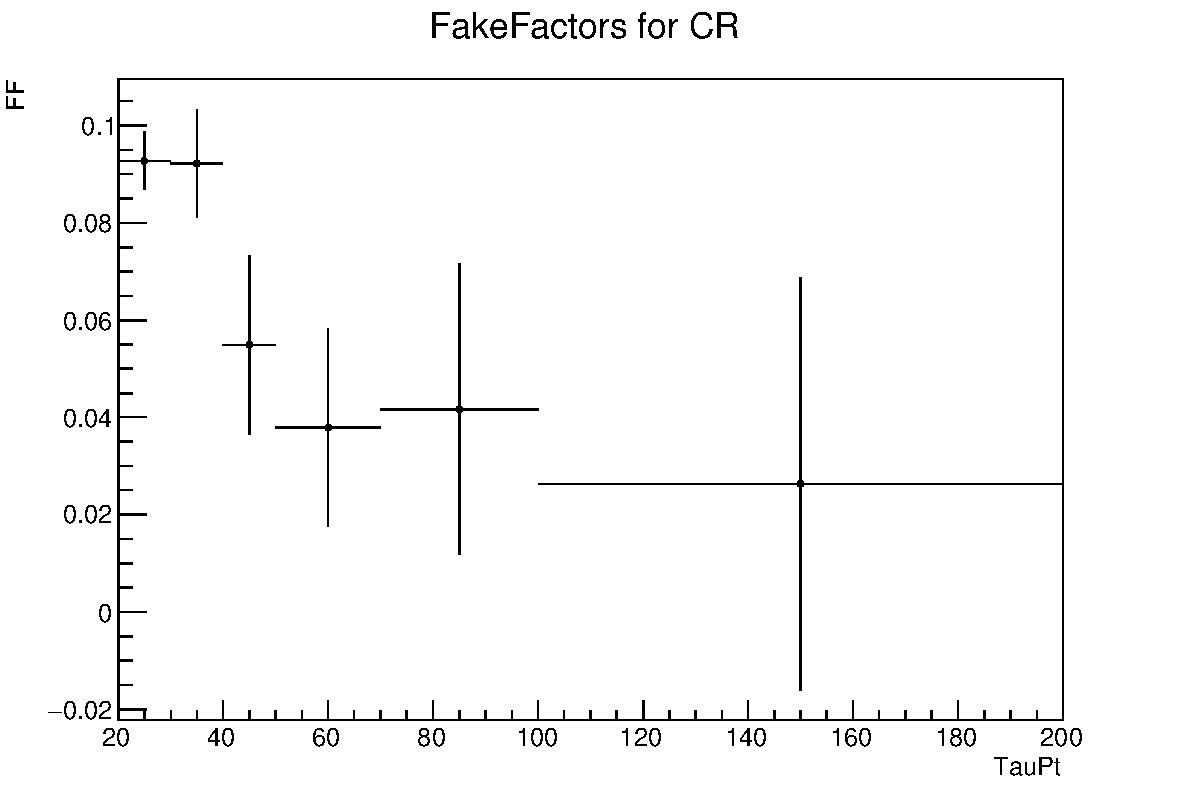
\includegraphics[width=.4\textwidth]{figures/lephadFF/SLT/FF_All_Preselection_Np3_CR_2tag_TauPt} \\
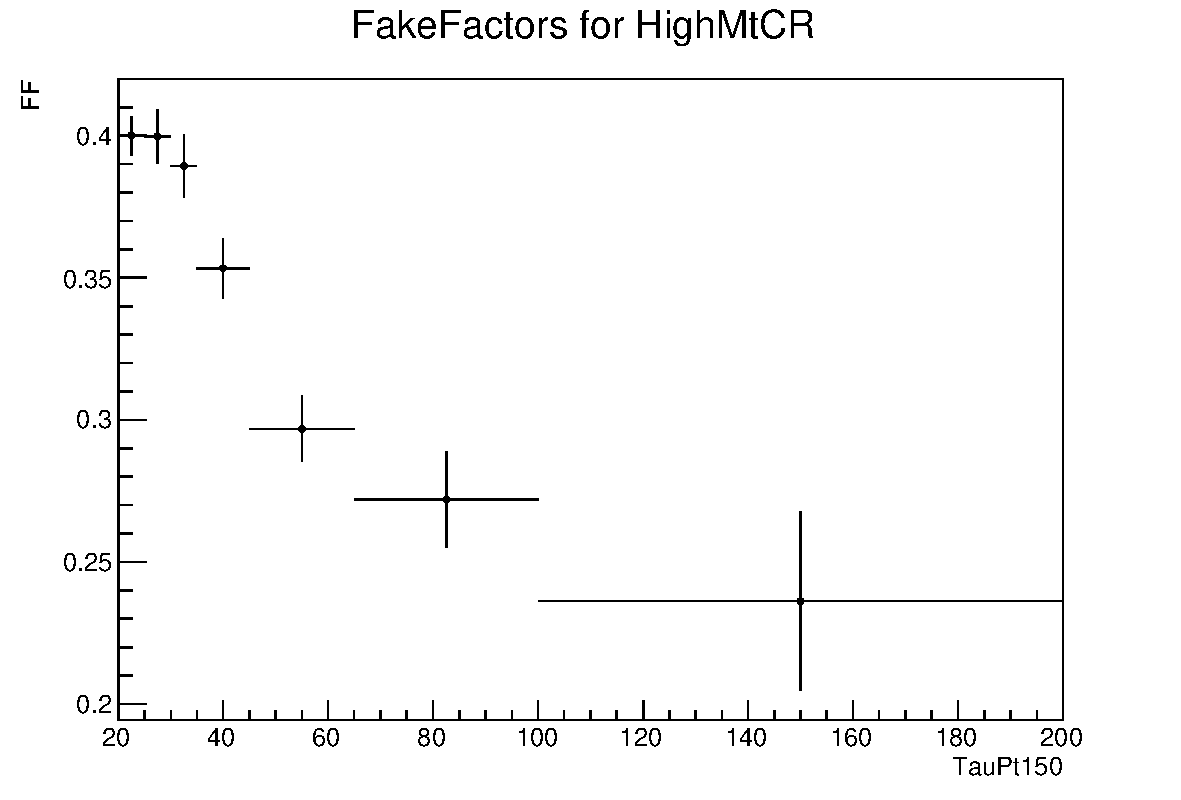
\includegraphics[width=.4\textwidth]{figures/lephadFF/SLT/FF_All_Preselection_Np1_HighMtCR_2tag_TauPt150}
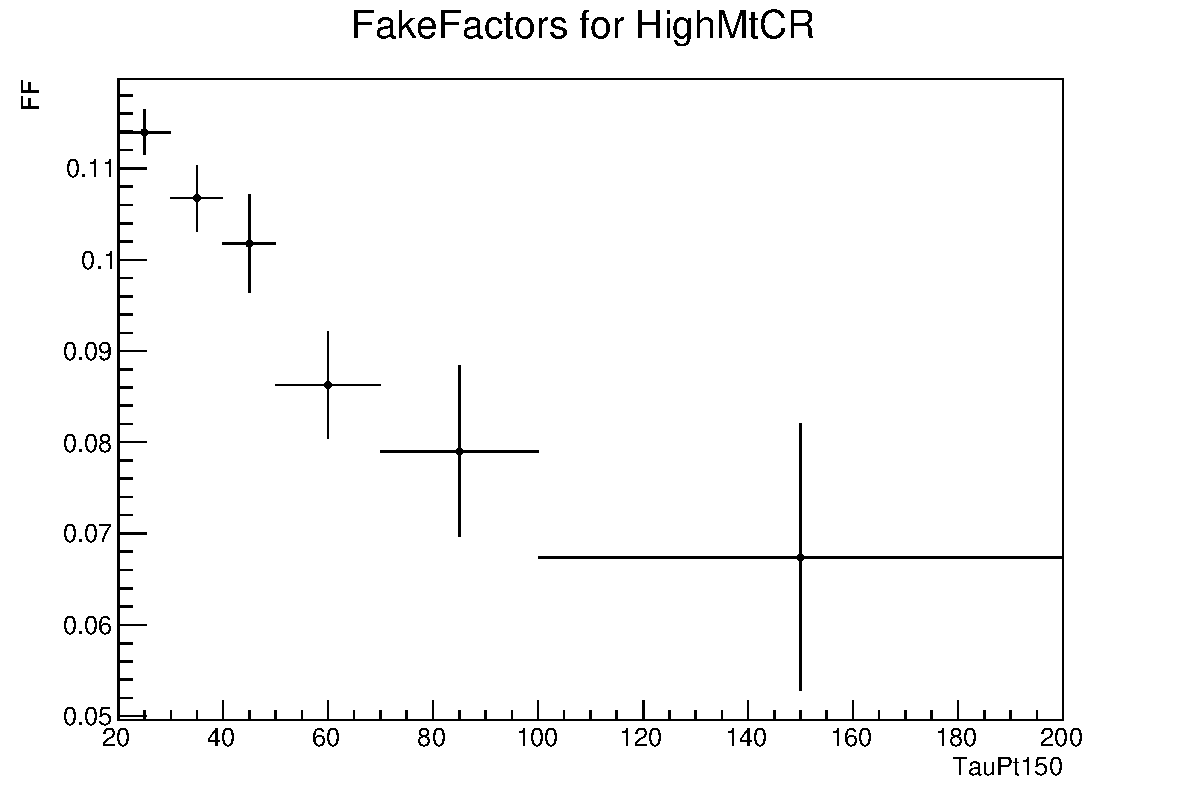
\includegraphics[width=.4\textwidth]{figures/lephadFF/SLT/FF_All_Preselection_Np3_HighMtCR_2tag_TauPt150}\\
\caption{Fake-factors for 1-prong (left) and 3-prong (right) \tauhad candidates for multi-jet (top) and \ttbar processes (bottom) for the \lephad SLT category.}
\label{fig:SLT_FF}
\end{figure}

\begin{figure}
\centering
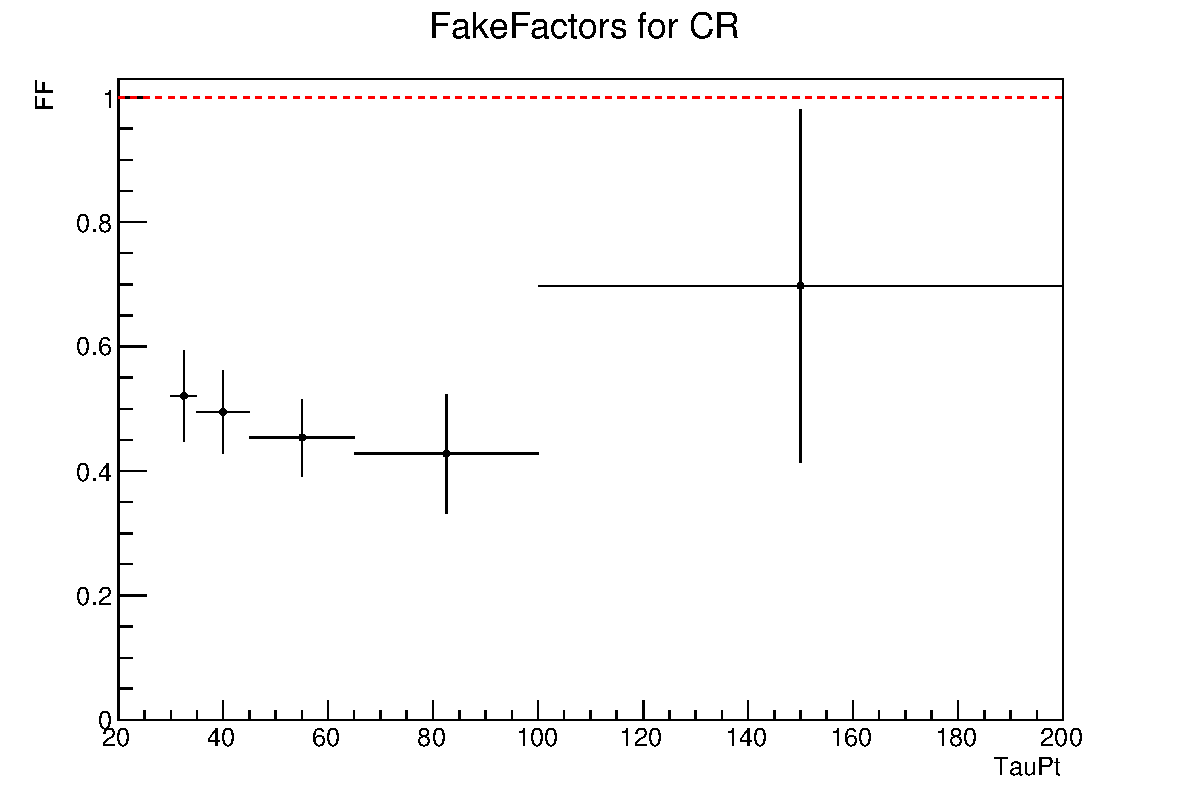
\includegraphics[width=.4\textwidth]{figures/lephadFF/LTT/FF_All_Preselection_Np1_CR_2tag_TauPt}
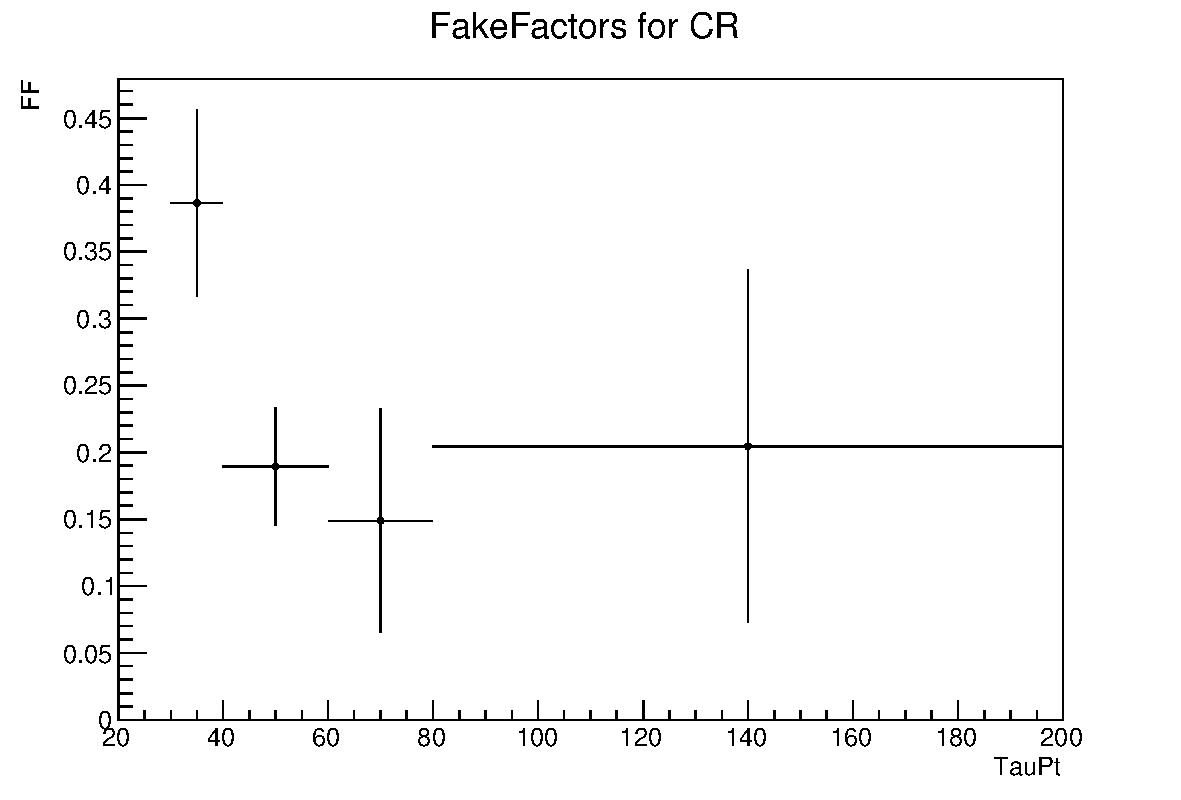
\includegraphics[width=.4\textwidth]{figures/lephadFF/LTT/FF_All_Preselection_Np3_CR_2tag_TauPt} \\
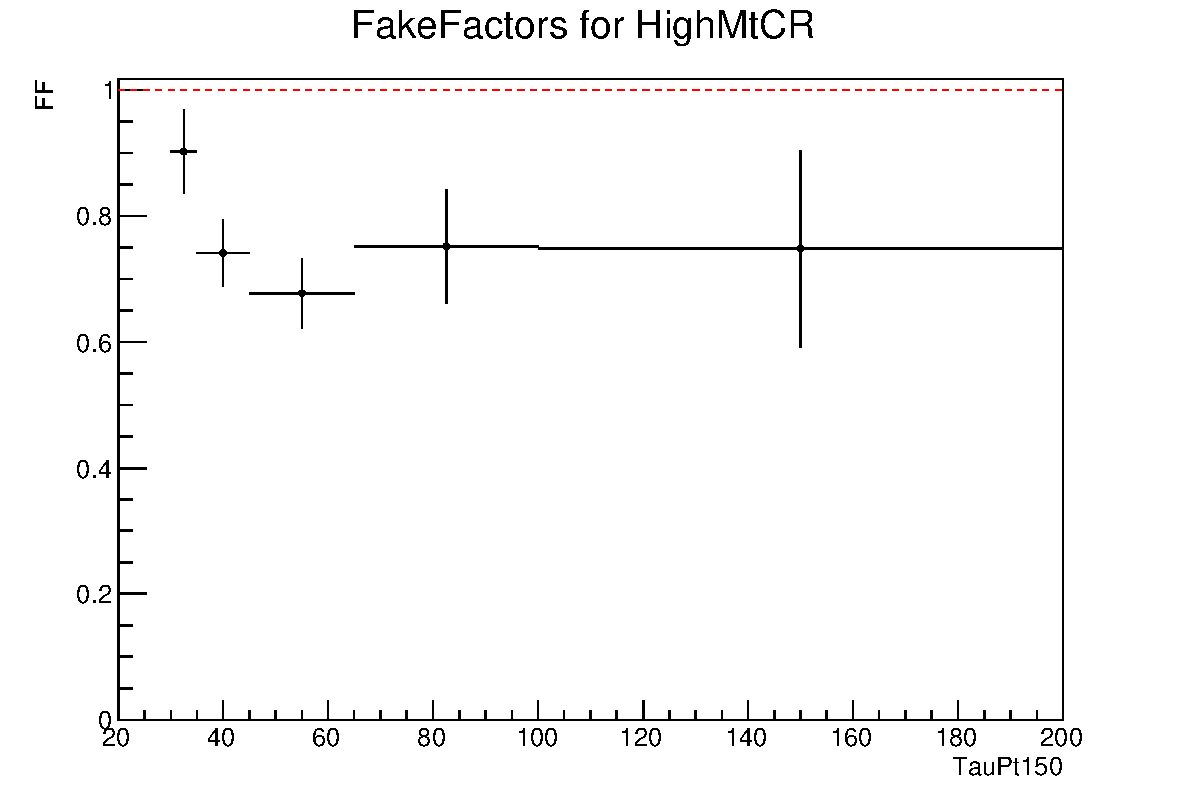
\includegraphics[width=.4\textwidth]{figures/lephadFF/LTT/FF_All_Preselection_Np1_HighMtCR_2tag_TauPt150}
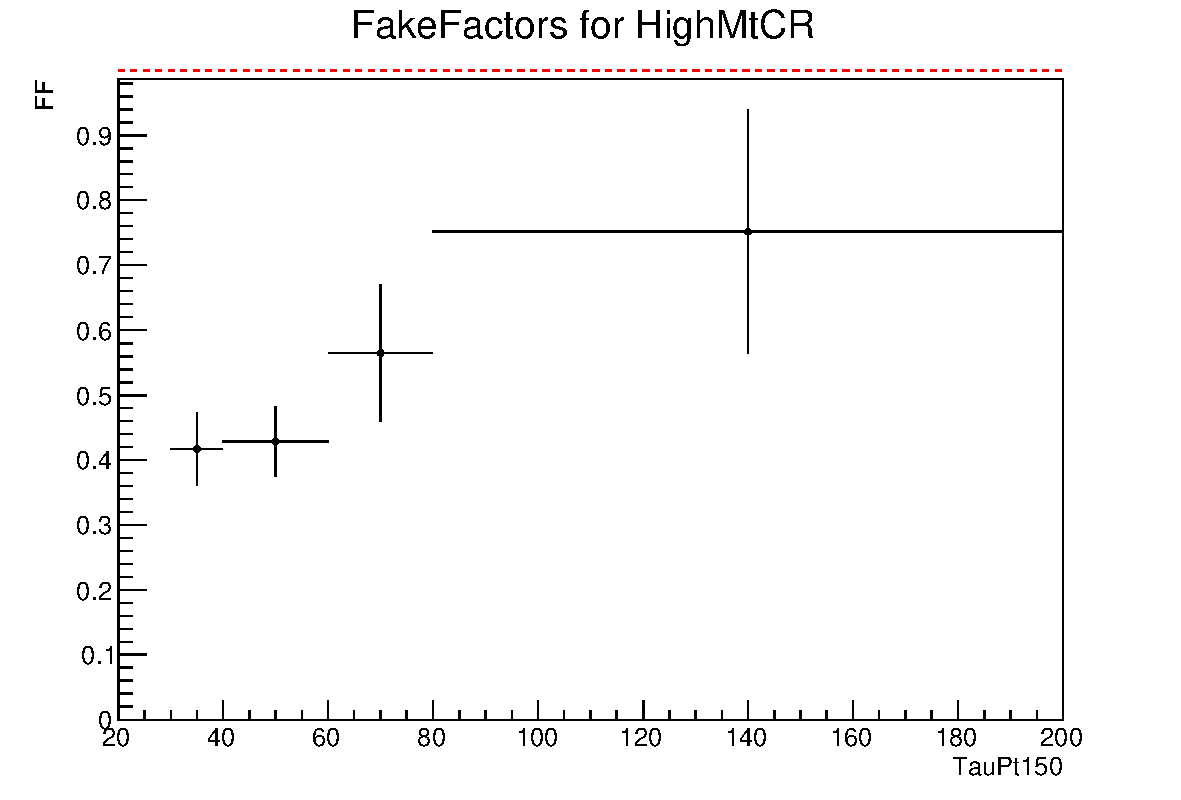
\includegraphics[width=.4\textwidth]{figures/lephadFF/LTT/FF_All_Preselection_Np3_HighMtCR_2tag_TauPt150}\\
\caption{Fake-factors for 1-prong (left) and 3-prong (right) \tauhad candidates for multi-jet (top) and \ttbar processes (bottom) for the \lephad LTT category.}
\label{fig:LTT_FF}
\end{figure}

\begin{figure}
\centering
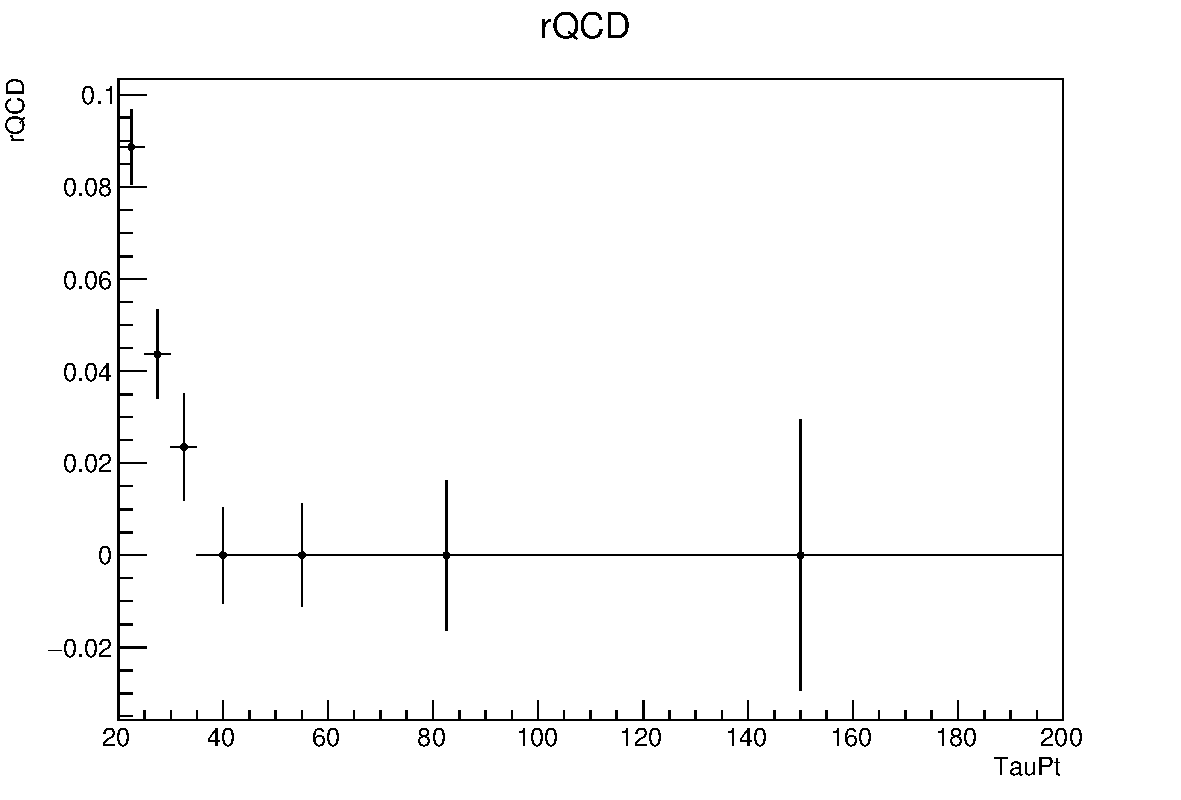
\includegraphics[width=.4\textwidth]{figures/lephadFF/SLT/rQCD_All_Preselection_Np1_Elec_CR_2tag_TauPt}
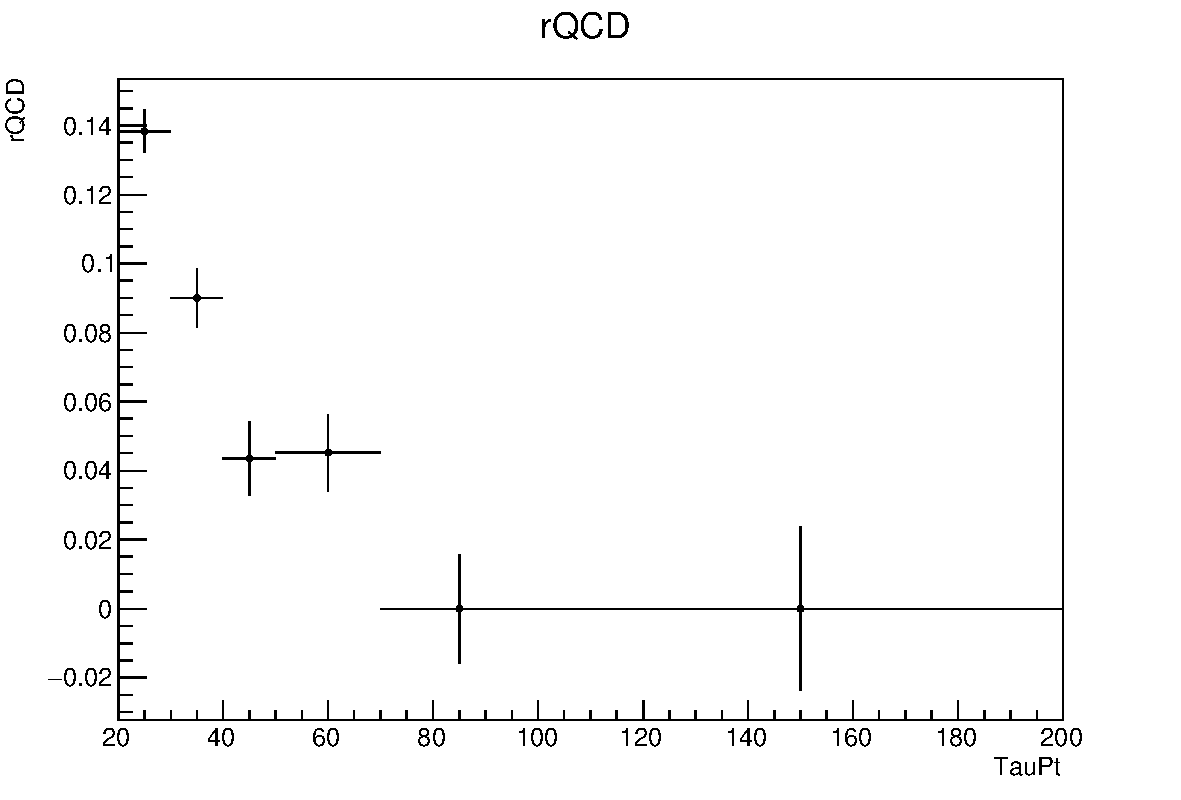
\includegraphics[width=.4\textwidth]{figures/lephadFF/SLT/rQCD_All_Preselection_Np3_Elec_CR_2tag_TauPt} \\
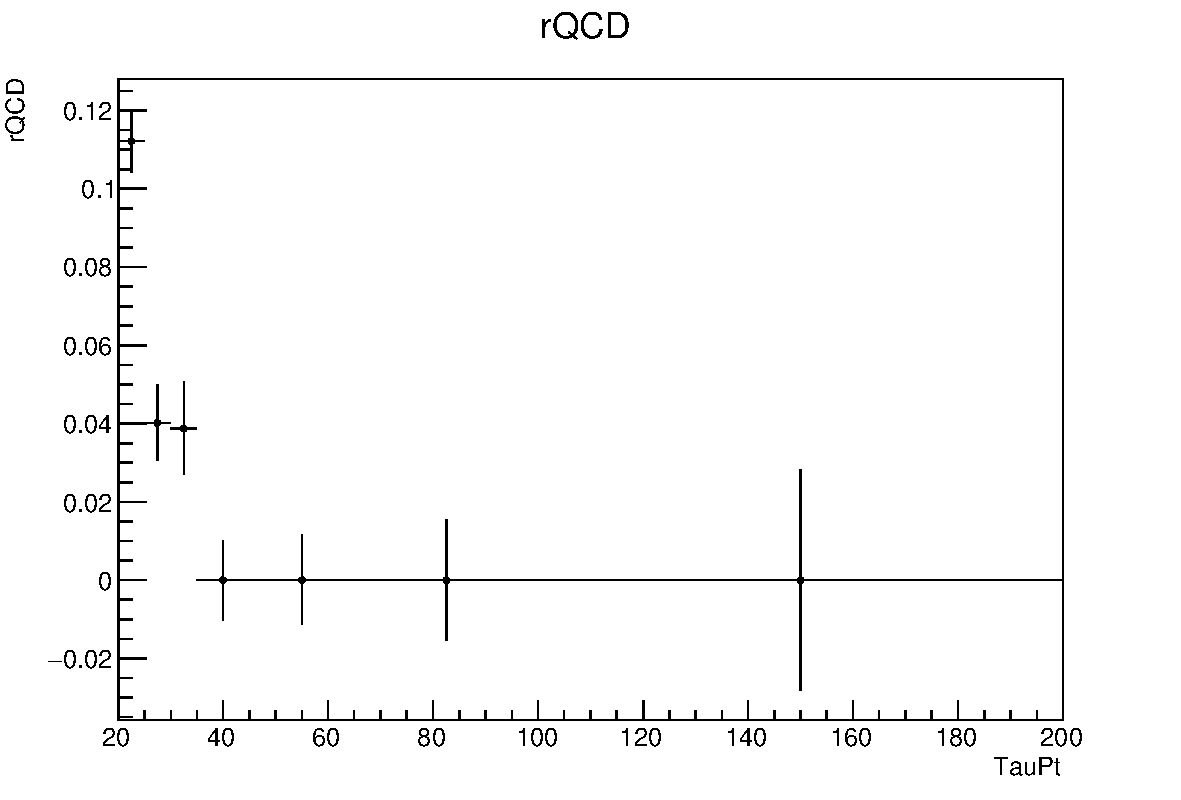
\includegraphics[width=.4\textwidth]{figures/lephadFF/SLT/rQCD_All_Preselection_Np1_Muon_CR_2tag_TauPt}
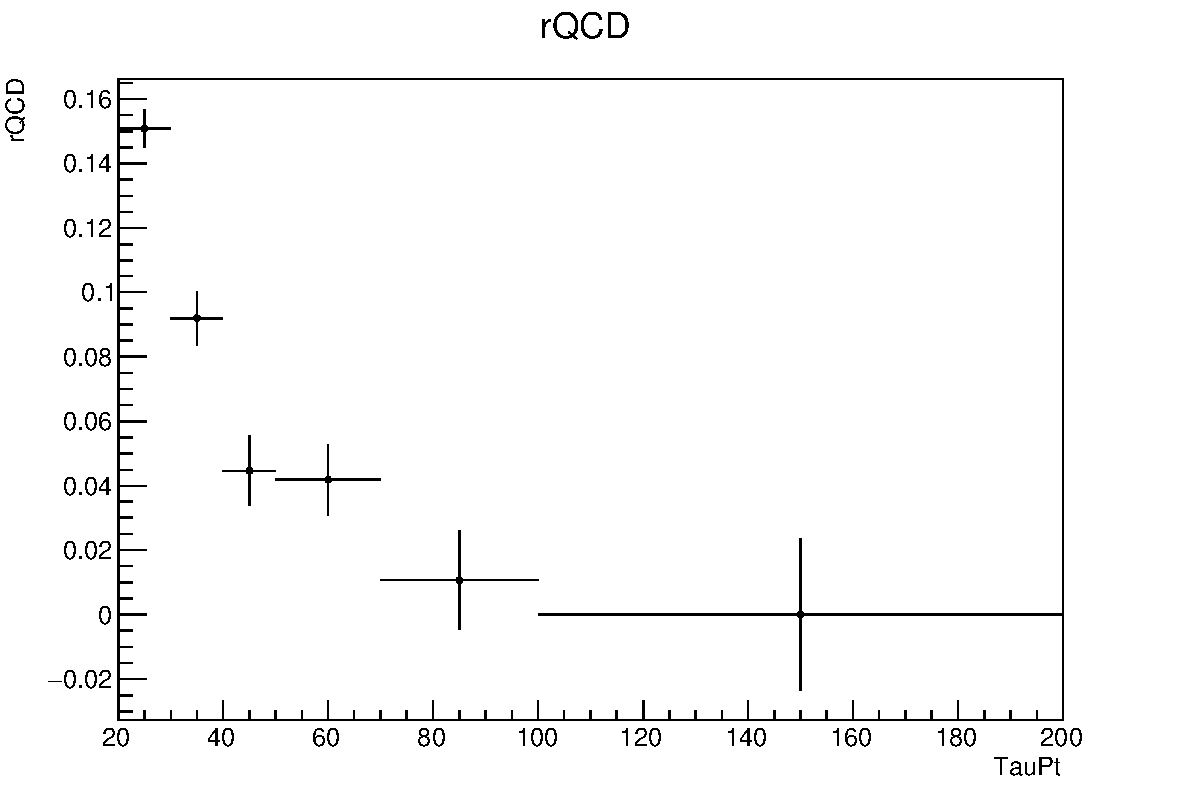
\includegraphics[width=.4\textwidth]{figures/lephadFF/SLT/rQCD_All_Preselection_Np3_Muon_CR_2tag_TauPt}\\
\caption{$\mathrm{r}_{\mathrm{QCD}}$ for 1-prong (left) and 3-prong (right) \tauhad candidates for $e\tauhad$ channel (top) and $\mu\tauhad$ (bottom) when requiring same-sign lepton-tau pairs for the \lephad SLT category.}
\label{fig:SLT_rQCD}
\end{figure}

\begin{figure}
\centering
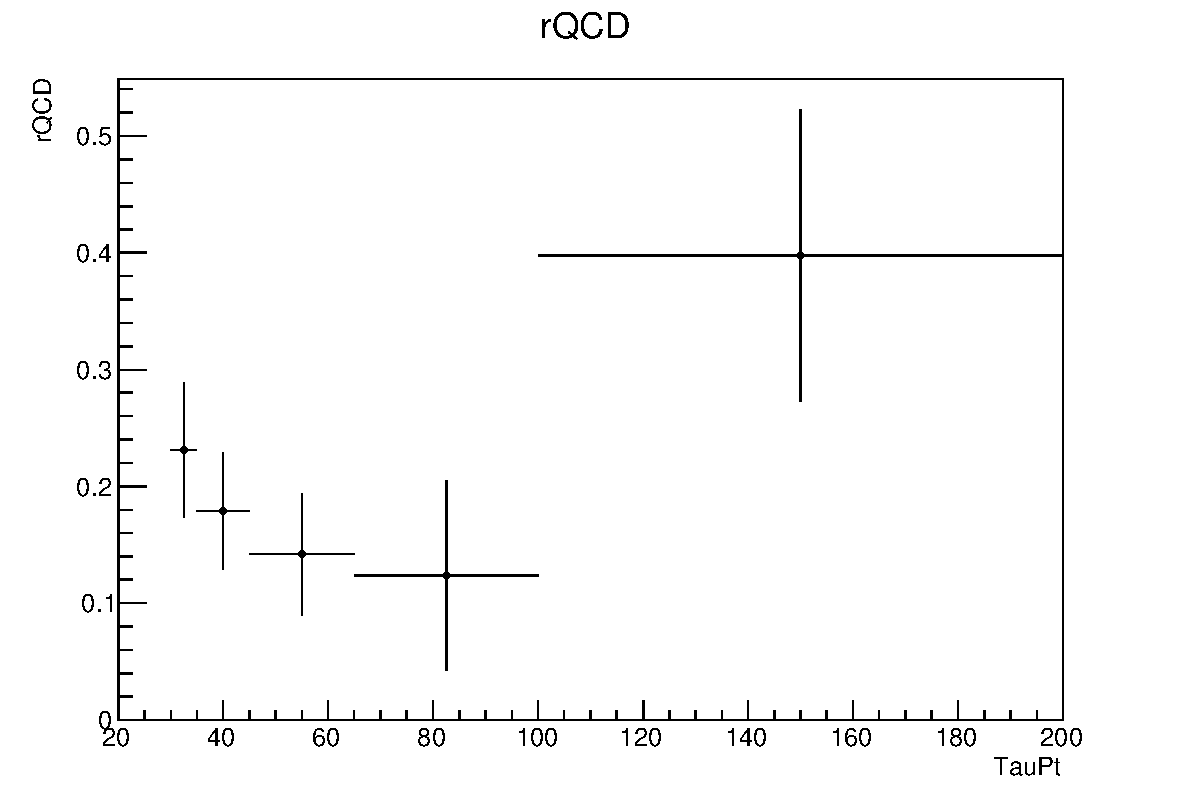
\includegraphics[width=.4\textwidth]{figures/lephadFF/LTT/rQCD_All_Preselection_Np1_Elec_CR_2tag_TauPt}
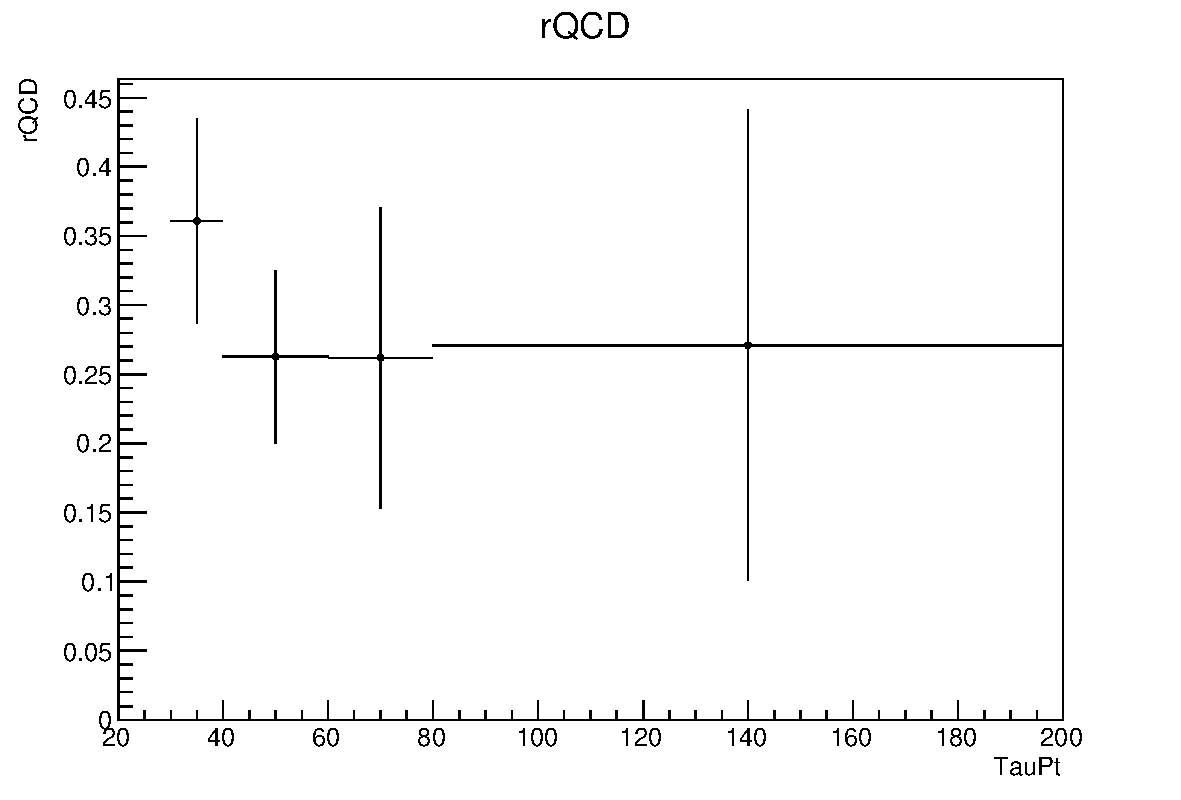
\includegraphics[width=.4\textwidth]{figures/lephadFF/LTT/rQCD_All_Preselection_Np3_Elec_CR_2tag_TauPt} \\
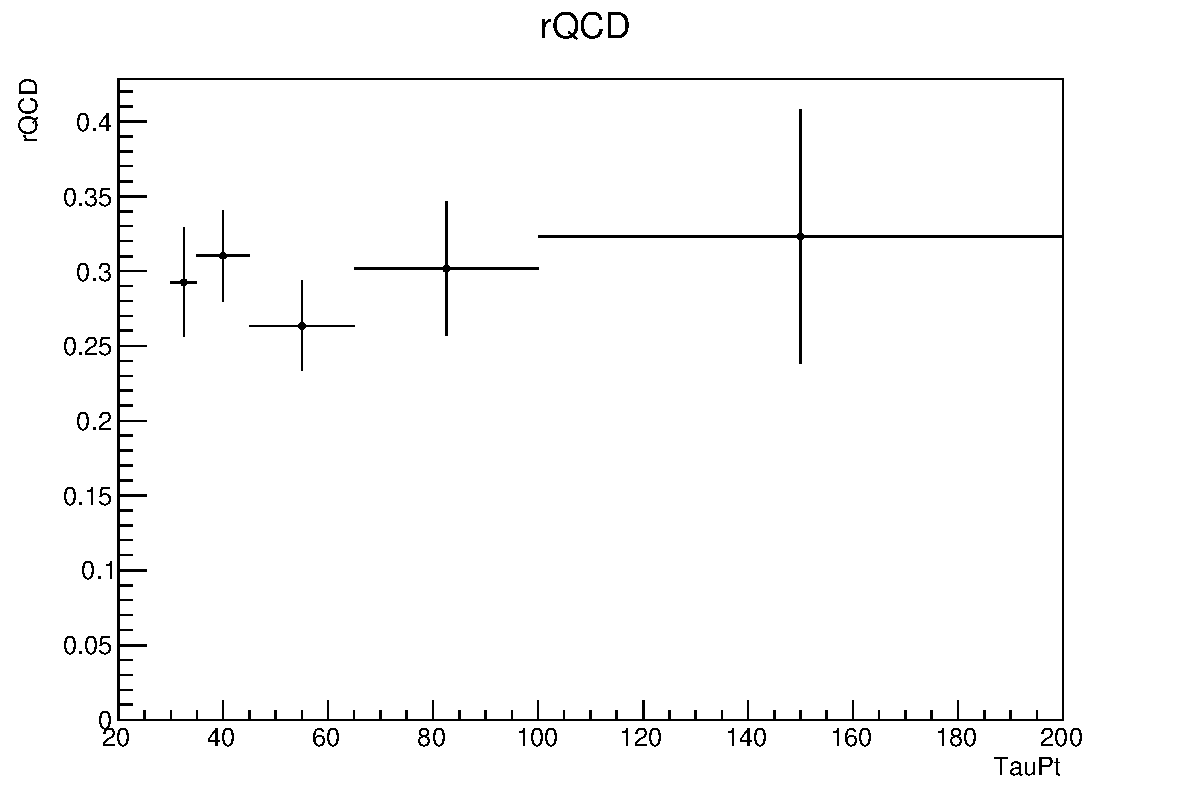
\includegraphics[width=.4\textwidth]{figures/lephadFF/LTT/rQCD_All_Preselection_Np1_Muon_CR_2tag_TauPt}
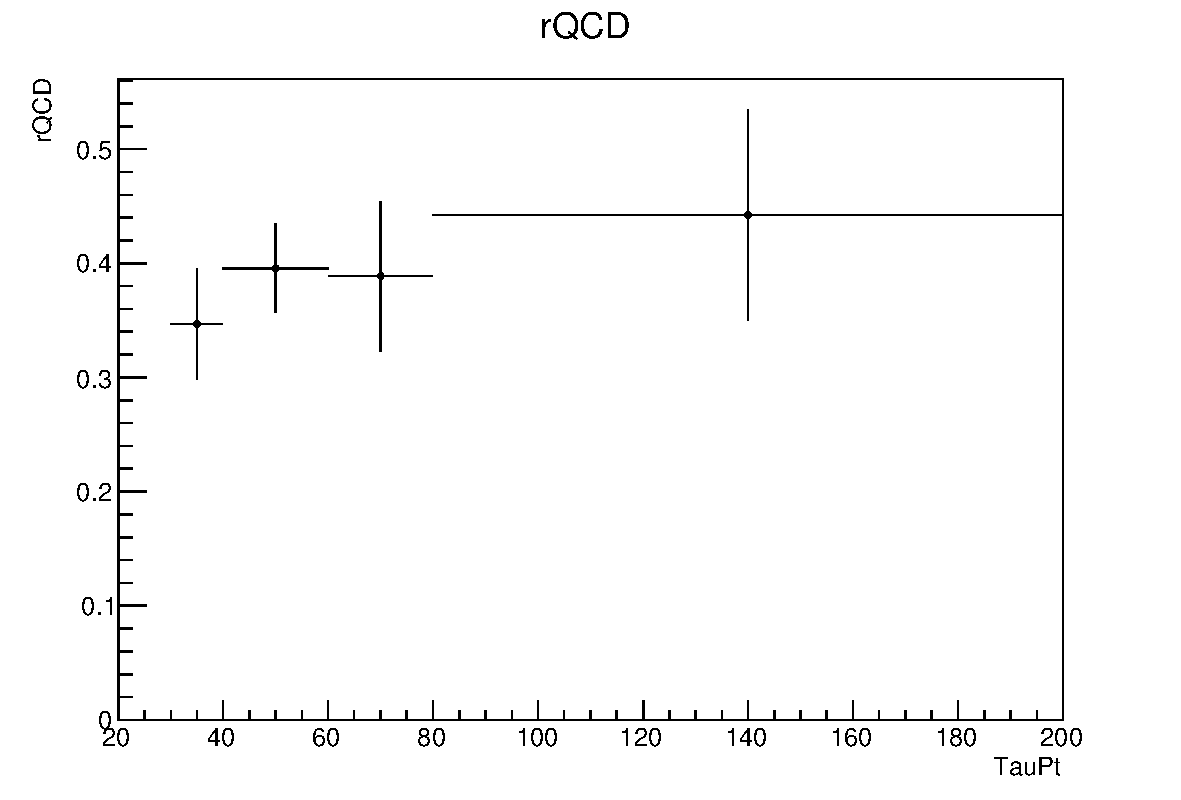
\includegraphics[width=.4\textwidth]{figures/lephadFF/LTT/rQCD_All_Preselection_Np3_Muon_CR_2tag_TauPt}\\
\caption{$\mathrm{r}_{\mathrm{QCD}}$ for 1-prong (left) and 3-prong (right) \tauhad candidates for $e\tauhad$ channel (top) and $\mu\tauhad$ (bottom) when requiring same-sign lepton-tau pairs for the \lephad LTT category.}
\label{fig:LTT_rQCD}
\end{figure}

Figure~\ref{fig:LH_MC_data_fakes} shows the comparison of the contribution of fakes as estimated using MC and using either the fake estimation or data with true $\tau$ backgrounds subtracted in the signal region and control region, respectively. As expected, the difference between MC and the data estimate is larger in the LTT channel, where the lower momentum events include more multi-jet events (for which MC is not available). This is shown with the analysis binning algorithm applied to the final discriminant for the non-resonant and several resonant mass points.

\begin{figure}
\centering
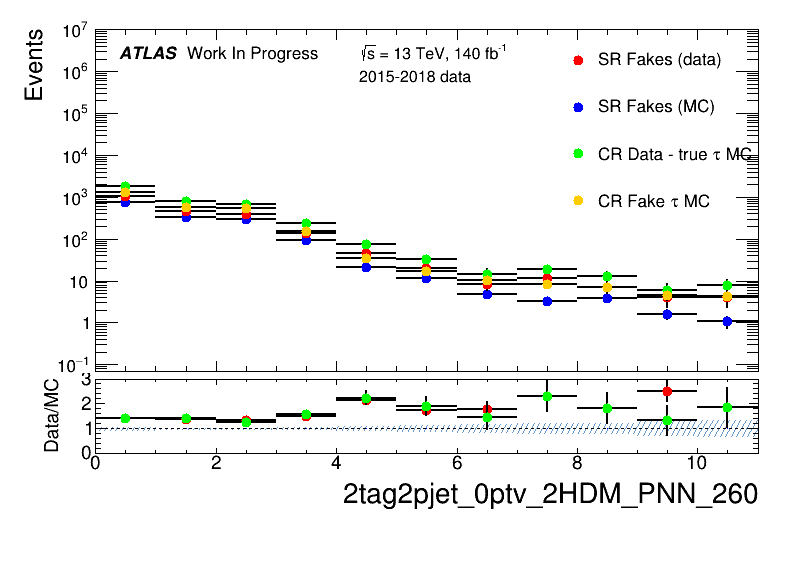
\includegraphics[width=.4\textwidth]{figures/lephadFF/LTT/2tag2pjet_0ptv_2HDM_PNN_260_LTT_CR_highPNN_fakes_log.png}
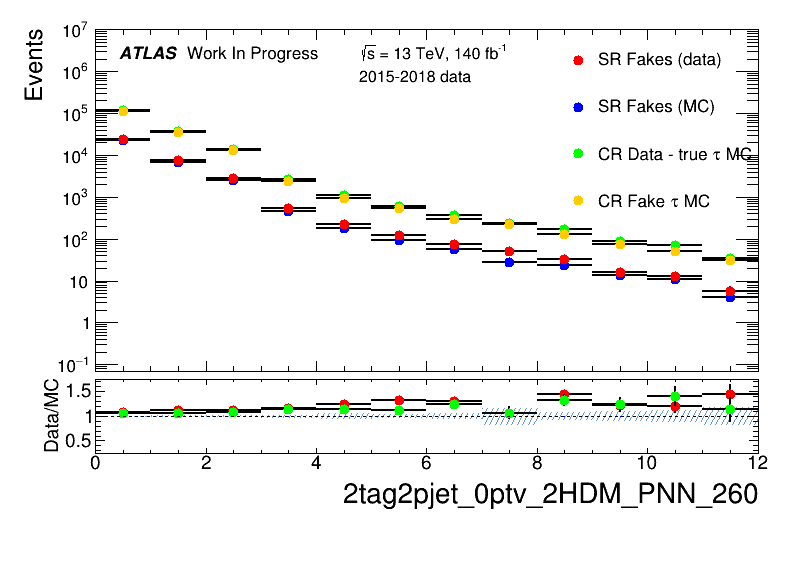
\includegraphics[width=.4\textwidth]{figures/lephadFF/SLT/2tag2pjet_0ptv_2HDM_PNN_260_SLT_CR_highPNN_fakes_log.png}\\
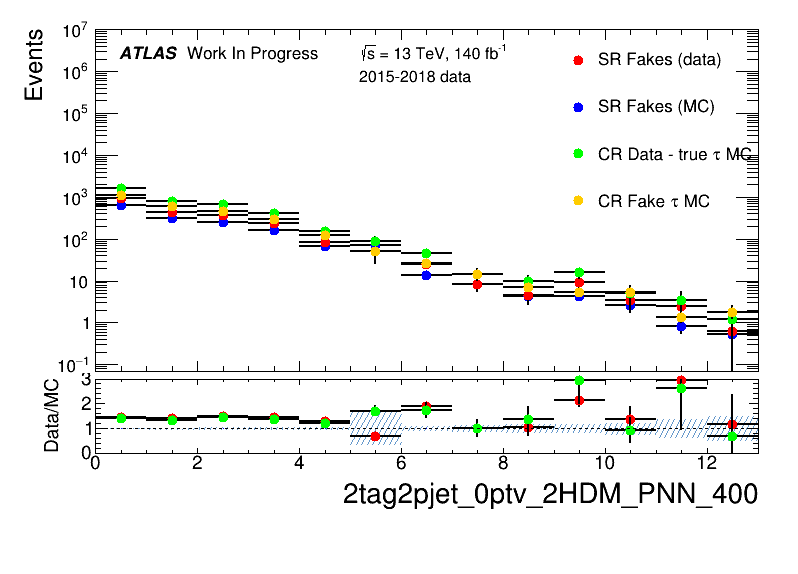
\includegraphics[width=.4\textwidth]{figures/lephadFF/LTT/2tag2pjet_0ptv_2HDM_PNN_400_LTT_CR_highPNN_fakes_log.png}
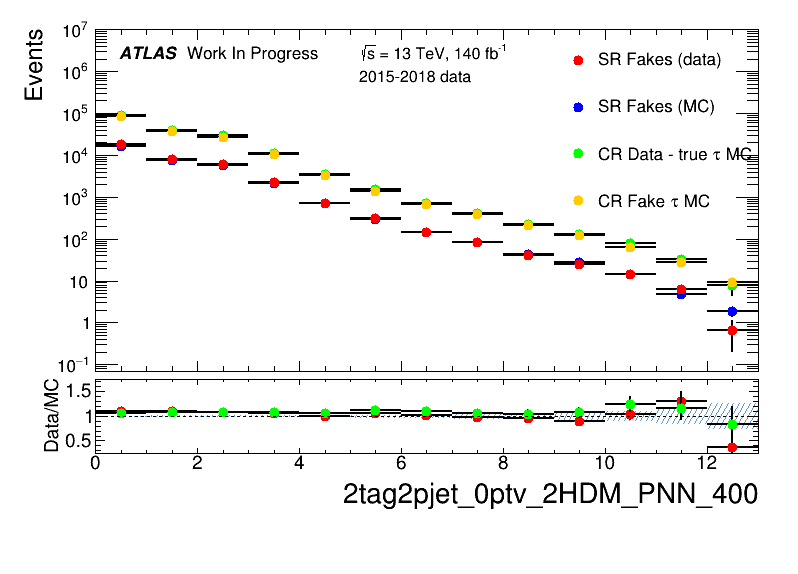
\includegraphics[width=.4\textwidth]{figures/lephadFF/SLT/2tag2pjet_0ptv_2HDM_PNN_400_SLT_CR_highPNN_fakes_log.png}\\
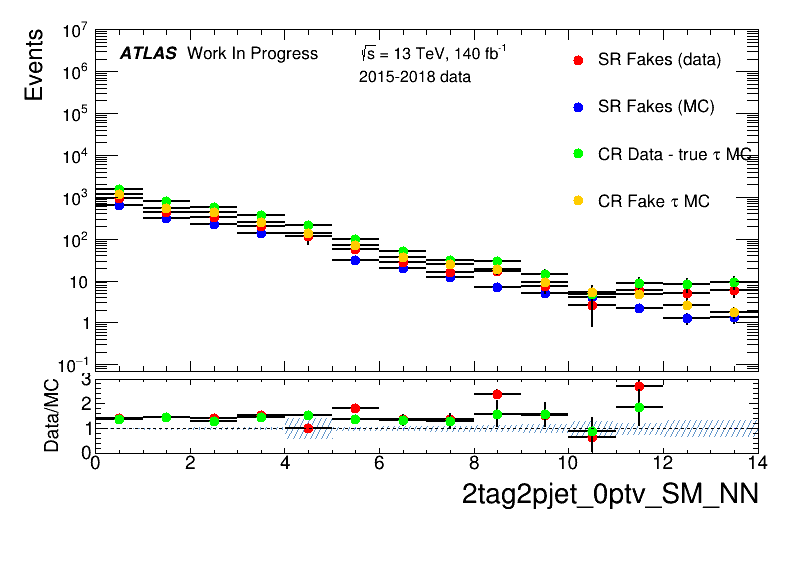
\includegraphics[width=.4\textwidth]{figures/lephadFF/LTT/2tag2pjet_0ptv_SM_NN_LTT_CR_highPNN_fakes_log.png}
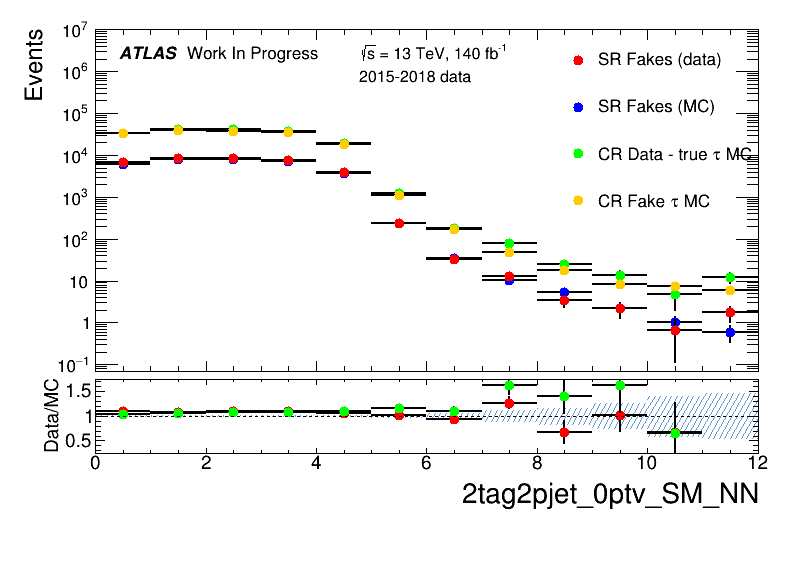
\includegraphics[width=.4\textwidth]{figures/lephadFF/SLT/2tag2pjet_0ptv_SM_NN_SLT_CR_highPNN_fakes_log.png}\\
\caption{A comparison of  the contribution of fakes as estimated using MC and using either the fake estimation or data with true $\tau$ backgrounds subtracted in the signal region and control region, respectively. Uncertainties are statistical only, and note that multi-jet contributions are included in the data estimates but not the MC. The distributions are the final discriminant for the 260 GeV (top) and 400 GeV (middle) resonant mass points, and the non-resonant discriminant (bottom) for the lepton-plus-tau trigger channel (left) and the single lepton trigger channel (right). }
\label{fig:LH_MC_data_fakes}
\end{figure} 

To validate the ability of the combined fake factor method to describe the PNN or NN shape, plots have been made using the fake factor method to estimate the combined multi-jet and $t\bar{t}/W$ contribution in validation regions. First, we have applied the combined fake factor method directly to the $\ttbar$ CR, as a closure test of the method, which can be seen in Fig.~\ref{fig:ttCR_val}. The next region is the high statistic and 
relatively background-enriched $0$-tag region, which is the same as the lephad signal region except for the requirement that there are 
no $b$-tagged jets.  This is shown in Fig.~\ref{fig:SLT_0tag} and Fig.~\ref{fig:LTT_0tag} for several mass hypotheses and for the single lepton and lepton-plus-tau trigger categories, respectively. In Fig.~\ref{fig:SLT_LTT_1tag} and Fig.~\ref{fig:SLT_LTT_1tag_NN}, a few distributions are also shown for a validation region closer to the signal region, the $1$-tag validation region, which requires the same selection as the signal region with the exception of requiring exactly one $b$-tagged jet. The background estimation appears to agree well with the observed distributions in these validation regions.

\begin{figure}
\centering
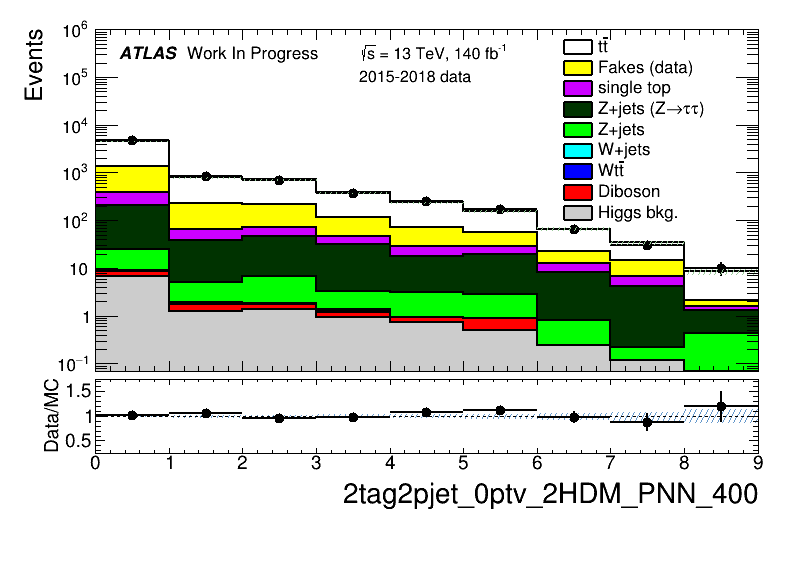
\includegraphics[width=.45\textwidth]{figures/lephadFF/LTT/2tag2pjet_0ptv_2HDM_PNN_400_SR_ALLFAKES_LTT_ttCR_noNeg_log.png}
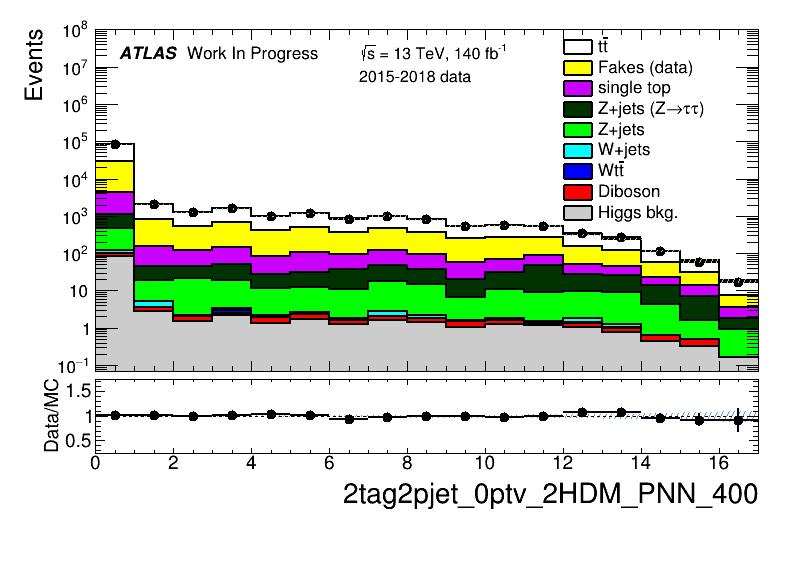
\includegraphics[width=.45\textwidth]{figures/lephadFF/SLT/2tag2pjet_0ptv_2HDM_PNN_400_SR_ALLFAKES_SLT_ttCR_noNeg_log.png}\\
\caption{The PNN distribution for the $m_{X} = 400$ GeV mass hypothesis in the signal-depleted $\ttbar$ CR where the $\ttbar$ FF are measured. This is a simple closure test.} 
\label{fig:ttCR_val}
\end{figure}



\begin{figure}
\centering
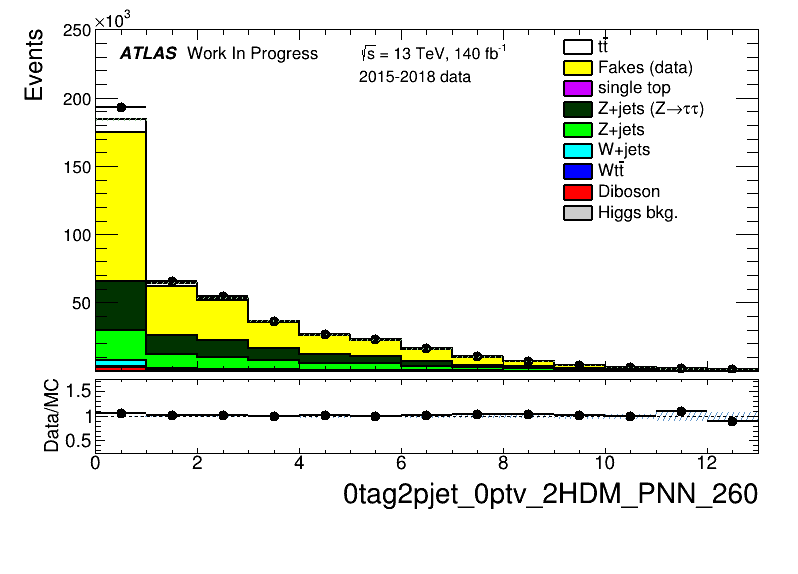
\includegraphics[width=.45\textwidth]{figures/lephadFF/SLT/0tag2pjet_0ptv_2HDM_PNN_260_SLT_ALLFAKES_Bulb_noNeg_lin.png}
\includegraphics[width=.45\textwidth]{figures/lephadFF/SLT/0tag2pjet_0ptv_2HDM_PNN_260_SLT_ALLFAKES_Bulb_noNeg_log.png}\\
\includegraphics[width=.45\textwidth]{figures/lephadFF/SLT/0tag2pjet_0ptv_2HDM_PNN_400_SLT_ALLFAKES_Bulb_noNeg_lin.png}
\includegraphics[width=.45\textwidth]{figures/lephadFF/SLT/0tag2pjet_0ptv_2HDM_PNN_400_SLT_ALLFAKES_Bulb_noNeg_log.png}\\
\includegraphics[width=.45\textwidth]{figures/lephadFF/SLT/0tag2pjet_0ptv_2HDM_PNN_1000_SLT_ALLFAKES_Bulb_noNeg_lin.png}
\includegraphics[width=.45\textwidth]{figures/lephadFF/SLT/0tag2pjet_0ptv_2HDM_PNN_1000_SLT_ALLFAKES_Bulb_noNeg_log.png}\\
\includegraphics[width=.45\textwidth]{figures/lephadFF/SLT/0tag2pjet_0ptv_SM_NN_SLT_ALLFAKES_Bulb_noNeg_lin.png}
\includegraphics[width=.45\textwidth]{figures/lephadFF/SLT/0tag2pjet_0ptv_SM_NN_SLT_ALLFAKES_Bulb_noNeg_log.png}
\caption{The PNN distribution for the $m_{X} = 260$, $400$, and $1000$ GeV mass hypotheses and the non-resonant NN distribution in the $0$-tag validation region of the single lepton trigger category in (left) linear and (right) log scale. The binning is defined using the same algorithm as is used for the signal region in the final fit, and normalization factors are used for $Z+HF$ (1.33) and $\ttbar$ (0.95).}
\label{fig:SLT_0tag}
\end{figure}    

\begin{figure}
\centering
\includegraphics[width=.45\textwidth]{figures/lephadFF/LTT/0tag2pjet_0ptv_2HDM_PNN_260_LTT_ALLFAKES_Bulb_noNeg_lin.png}
\includegraphics[width=.45\textwidth]{figures/lephadFF/LTT/0tag2pjet_0ptv_2HDM_PNN_260_LTT_ALLFAKES_Bulb_noNeg_log.png}\\
\includegraphics[width=.45\textwidth]{figures/lephadFF/LTT/0tag2pjet_0ptv_2HDM_PNN_400_LTT_ALLFAKES_Bulb_noNeg_lin.png}
\includegraphics[width=.45\textwidth]{figures/lephadFF/LTT/0tag2pjet_0ptv_2HDM_PNN_400_LTT_ALLFAKES_Bulb_noNeg_log.png}\\
\includegraphics[width=.45\textwidth]{figures/lephadFF/LTT/0tag2pjet_0ptv_2HDM_PNN_1000_LTT_ALLFAKES_Bulb_noNeg_lin.png}
\includegraphics[width=.45\textwidth]{figures/lephadFF/LTT/0tag2pjet_0ptv_2HDM_PNN_1000_LTT_ALLFAKES_Bulb_noNeg_log.png}\\
\includegraphics[width=.45\textwidth]{figures/lephadFF/LTT/0tag2pjet_0ptv_SM_NN_LTT_ALLFAKES_Bulb_noNeg_lin.png}
\includegraphics[width=.45\textwidth]{figures/lephadFF/LTT/0tag2pjet_0ptv_SM_NN_LTT_ALLFAKES_Bulb_noNeg_log.png}
\caption{The PNN distribution for the $m_{X} = 260$, $400$, and $1000$ GeV mass hypotheses and the non-resonant NN distribution in the $0$-tag validation region of the lepton-plus-tau trigger category in (left) linear and (right) log scale. The binning is defined using the same algorithm as is used for the signal region in the final fit, and normalization factors are used for $Z+HF$ (1.33) and $\ttbar$ (0.95).}
\label{fig:LTT_0tag}
\end{figure}    

\begin{figure}   
\centering
\includegraphics[width=.45\textwidth]{figures/lephadFF/SLT/1tag2pjet_0ptv_2HDM_PNN_260_SLT_ALLFAKES_Bulb_noNeg_lin.png}
\includegraphics[width=.45\textwidth]{figures/lephadFF/SLT/1tag2pjet_0ptv_2HDM_PNN_260_SLT_ALLFAKES_Bulb_noNeg_log.png}\\
\includegraphics[width=.45\textwidth]{figures/lephadFF/SLT/1tag2pjet_0ptv_2HDM_PNN_400_SLT_ALLFAKES_Bulb_noNeg_lin.png}
\includegraphics[width=.45\textwidth]{figures/lephadFF/SLT/1tag2pjet_0ptv_2HDM_PNN_400_SLT_ALLFAKES_Bulb_noNeg_log.png}\\
\includegraphics[width=.45\textwidth]{figures/lephadFF/LTT/1tag2pjet_0ptv_2HDM_PNN_260_LTT_ALLFAKES_Bulb_noNeg_lin.png}
\includegraphics[width=.45\textwidth]{figures/lephadFF/LTT/1tag2pjet_0ptv_2HDM_PNN_260_LTT_ALLFAKES_Bulb_noNeg_log.png}\\
\includegraphics[width=.45\textwidth]{figures/lephadFF/LTT/1tag2pjet_0ptv_2HDM_PNN_400_LTT_ALLFAKES_Bulb_noNeg_lin.png}
\includegraphics[width=.45\textwidth]{figures/lephadFF/LTT/1tag2pjet_0ptv_2HDM_PNN_400_LTT_ALLFAKES_Bulb_noNeg_log.png}\\
\caption{The PNN distribution for the $m_{X} = 260$ and $400$ GeV mass hypotheses in the $1$-tag validation region of the (top) single lepton trigger category and (bottom) lepton-plus-tau trigger category in (left) linear and (right) log scale. The binning is defined using the same algorithm as is used for the signal region in the final fit, and normalization factors are used for $Z+HF$ (1.33) and $\ttbar$ (0.95).}
\label{fig:SLT_LTT_1tag}
\end{figure}

\begin{figure}
\centering
\includegraphics[width=.45\textwidth]{figures/lephadFF/SLT/1tag2pjet_0ptv_SM_NN_SLT_ALLFAKES_Bulb_noNeg_lin.png}
\includegraphics[width=.45\textwidth]{figures/lephadFF/SLT/1tag2pjet_0ptv_SM_NN_SLT_ALLFAKES_Bulb_noNeg_log.png}\\
\includegraphics[width=.45\textwidth]{figures/lephadFF/LTT/1tag2pjet_0ptv_SM_NN_LTT_ALLFAKES_Bulb_noNeg_lin.png}
\includegraphics[width=.45\textwidth]{figures/lephadFF/LTT/1tag2pjet_0ptv_SM_NN_LTT_ALLFAKES_Bulb_noNeg_log.png}\\
\caption{The PNN distribution for the non-resonant signal hypothesis in the $1$-tag validation region of the (top) single lepton trigger category and (bottom) lepton-plus-tau trigger category in (left) linear and (right) log scale. The binning is defined using the same algorithm as is used for the signal region in the final fit, and normalization factors are used for $Z+HF$ (1.33) and $\ttbar$ (0.95).}
\label{fig:SLT_LTT_1tag_NN}
\end{figure}

It was also requested to see what the SM NN plots looked like in the 0-tag and 1-tag regions with the exact binning used in the signal region, rather than the a binning defined by the algorithm that is used in the signal region.  This binning is not derived from the distributions in the 0-tag and 1-tag region at all, but is instead an example of what a binning derived in a different region would look like in the validation regions.  This is shown in Fig.~\ref{fig:SLT_LTT_0tag_SR} and Fig.~\ref{fig:SLT_LTT_1tag_SR}.  

\begin{figure}
\centering
\includegraphics[width=.45\textwidth]{figures/lephadFF/SLT/0tag2pjet_0ptv_SM_NN_SLT_ALLFAKES_Bulb_SRbinning_lin.png}
\includegraphics[width=.45\textwidth]{figures/lephadFF/SLT/0tag2pjet_0ptv_SM_NN_SLT_ALLFAKES_Bulb_SRbinning_log.png}\\
\includegraphics[width=.45\textwidth]{figures/lephadFF/LTT/0tag2pjet_0ptv_SM_NN_LTT_ALLFAKES_Bulb_SRbinning_lin.png}
\includegraphics[width=.45\textwidth]{figures/lephadFF/LTT/0tag2pjet_0ptv_SM_NN_LTT_ALLFAKES_Bulb_SRbinning_log.png}\\
\caption{The NN distribution for the non-resonant signal hypothesis in the $0$-tag validation region of the (top) single lepton trigger category and (bottom) lepton-plus-tau trigger category in (left) linear and (right) log scale. The binning is exactly the same as is used for the signal region in the final fit, and normalization factors are used for $Z+HF$ (1.33) and $\ttbar$ (0.95).}
\label{fig:SLT_LTT_0tag_SR}
\end{figure}

\begin{figure}
\centering
\includegraphics[width=.45\textwidth]{figures/lephadFF/SLT/1tag2pjet_0ptv_SM_NN_SLT_ALLFAKES_Bulb_SRbinning_lin.png}
\includegraphics[width=.45\textwidth]{figures/lephadFF/SLT/1tag2pjet_0ptv_SM_NN_SLT_ALLFAKES_Bulb_SRbinning_log.png}\\
\includegraphics[width=.45\textwidth]{figures/lephadFF/LTT/1tag2pjet_0ptv_SM_NN_LTT_ALLFAKES_Bulb_SRbinning_lin.png}
\includegraphics[width=.45\textwidth]{figures/lephadFF/LTT/1tag2pjet_0ptv_SM_NN_LTT_ALLFAKES_Bulb_SRbinning_log.png}\\
\caption{The NN distribution for the non-resonant signal hypothesis in the $1$-tag validation region of the (top) single lepton trigger category and (bottom) lepton-plus-tau trigger category in (left) linear and (right) log scale. The binning is exactly the same as is used for the signal region in the final fit, and normalization factors are used for $Z+HF$ (1.33) and $\ttbar$ (0.95).}
\label{fig:SLT_LTT_1tag_SR}
\end{figure}


\FloatBarrier

